\chapter[O$^+$ Approximation]{Large-Scale Environmental Dependence of Chemical Abundances in Dwarf Galaxies and Implications for Connecting Star Formation and Halo Mass}\label{ch:Paper3}


This chapter has been submitted to the \emph{Astrophysical Journal} by Kelly A. 
Douglass, Michael S. Vogeley, and Renyue Cen; it will be referenced as Douglass 
et. al (2017, submitted).



%%%%%%%%%%%%%%%%%%%%%%%%%%%%%%%%%%%%%%%%%%%%%%%%%%%%%%%%%%%%%%%%%%%%%%%%%%%%%%%%
%
%    ABSTRACT
%
%%%%%%%%%%%%%%%%%%%%%%%%%%%%%%%%%%%%%%%%%%%%%%%%%%%%%%%%%%%%%%%%%%%%%%%%%%%%%%%%
\begin{chapabstract}
We study how the void environment affects the chemical evolution of galaxies in 
the universe by comparing the oxygen and nitrogen abundances of dwarf galaxies 
in voids with dwarf galaxies in denser regions.  Using spectroscopic 
observations from the Sloan Digital Sky Survey Data Release 7, we estimate the 
oxygen and nitrogen abundances of 993 void dwarf galaxies and 759 dwarf galaxies 
in denser regions.  We use the Direct $T_e$ method for calculating the gas-phase 
chemical abundances in the dwarf galaxies because it is best suited for low 
metallicity, low mass (dwarf) galaxies.  A substitute for the [\ion{O}{2}] 
$\lambda 3727$ doublet is developed, permitting oxygen abundance estimates of 
SDSS dwarf galaxies at all redshifts with the Direct $T_e$ method.  We find that 
void dwarf galaxies have slightly higher oxygen abundances ($\sim$7\%) than 
dwarf galaxies in denser environments.  The opposite trend is seen in both the 
nitrogen abundance and N/O ratio: void dwarf galaxies have slightly lower 
nitrogen abundances ($\sim$10\%) and lower N/O ratios ($\sim$17\%) than dwarf 
galaxies in denser regions.  Our mass-N/O relationship shows that the secondary 
production of nitrogen commences at a lower stellar mass in void dwarf 
star-forming galaxies than in dwarf star-forming galaxies in denser 
environments.  We also find that star-forming void dwarf galaxies have higher 
\ion{H}{1} masses than the star-forming dwarf galaxies in denser regions.  Our 
star-forming dwarf galaxy sample demonstrates a strong anti-correlation between 
the sSFR and N/O ratio, providing evidence that oxygen is produced in higher 
mass stars than those which synthesize nitrogen.  The lower N/O ratios and 
smaller stellar mass for secondary nitrogen production seen in void dwarf 
galaxies may indicate both delayed star formation as predicted by $\Lambda$CDM 
cosmology and a dependence of cosmic downsizing on the large-scale environment.  
The shift toward higher oxygen abundances and higher \ion{H}{1} masses in void 
dwarf galaxies might be evidence of larger ratios of dark matter halo mass to 
stellar mass in voids than in denser regions.
\end{chapabstract}


%%%%%%%%%%%%%%%%%%%%%%%%%%%%%%%%%%%%%%%%%%%%%%%%%%%%%%%%%%%%%%%%%%%%%%%%%%%%%%%%
%
%    INTRODUCTION
%
%%%%%%%%%%%%%%%%%%%%%%%%%%%%%%%%%%%%%%%%%%%%%%%%%%%%%%%%%%%%%%%%%%%%%%%%%%%%%%%%
\section{Introduction}


% Primary v. secondary production of nitrogen (reminder) & its influence on the CNO cycle
%% What would cause less nitrogen to be produced in void galaxies?
%Lower production rates of nitrogen relative to oxygen production in void dwarf 
%galaxies could be a consequence of the retarded star formation predicted for 
%dwarf galaxies in voids by the $\Lambda$CDM cosmology.  In stellar 
%nucleosynthesis, there are two main classes of elements: primary and secondary.  
%Primary elements are those produced which do not depend on the quantity of any 
%other elements present in the star (excepting hydrogen, of course).  On the 
%other hand, secondary elements can be synthesized only when other elements are 
%already present in the star at the time of its birth.  Oxygen is a primary 
%element in stellar nucleosynthesis.  There is evidence 
%\textcolor{red}{(SOURCES)} to suggest that nitrogen behaves as both a primary 
%and secondary element.  The main source of nitrogen production is during the CNO 
%cycle, where carbon is needed as a catalyst for the reactions to begin.  If a 
%star is born with enough carbon, then it commences the CNO cycle much earlier 
%than in a star created with only hydrogen (or with only trace amounts of 
%carbon).  If star formation is retarded in void dwarf galaxies, then there are 
%fewer of the heavy elements that have been produced up to this point in time.  
%As a result, the stars that are created have less carbon initially present in 
%the star than in stars within wall dwarf galaxies, and less nitrogen will be 
%produced.  Fig. \ref{fig:N_1sig} shows evidence of this fact --- there is 
%slightly less nitrogen in void dwarf galaxies than in the dwarf galaxies in more 
%dense environments.  


% Prominence of voids in large-scale structure 
% (refs up through Pan et al., other recent void catalogs, ref to van Weygaert review)
Galactic redshift surveys have revealed that the large-scale distribution of 
galaxies is similar to a three-dimensional cosmic web \citep{Bond96}, with thin 
filaments of galaxies connecting galaxy clusters separated by voids (large, 
underdense areas which fill more than 60\% of space).  The voids first 
identified in early surveys \citep[e.g.,][]{Gregory78,Kirshner81,deLapparent86} 
have proven to be a universal feature of large-scale structure.  Analyses of the 
Sloan Digital Sky Survey \citep{Abazajian09,Ahn12} have produced catalogs of 
$10^3$ voids \citep{Pan12,Sutter14}.  Cosmic voids are an essential component for 
understanding the role of a galaxy's environment on its formation and evolution 
\citep[see][for a review]{vandeWeygaert11}.  

% Influence of the large-scale environment on galaxy properties
%  - well-established morphology-density relation (refs starting with Dressler 1980; Postman & Geller 1984)
%  - morphology-luminosity-density (Park et al. 2005?)
%  - evidence that trend continues into voids, where galaxies are found to be bluer, later type, higher sSFR (Rojas et al. 2004, 2005, who attribute this to availability of cool gas to feed star formation, and other refs)
%  - shift of void galaxy luminosity function (Hoyle et al.; Moorman et al.)
%  - consistent with shift of dark matter halo mass function (Goldberg et al.)
%  - investigations of HI properties of void galaxies (Kreckel et al., Moorman et al.)
%  - other refs to "Void galaxy survey" by Kreckel, van de Weygaert et al.
Extensive studies have been performed to understand the role of the environment 
in galaxy formation.  A strong relationship was found between a galaxy's 
morphology and the local density \citep{Dressler80,Postman84}, where the 
fraction of early-type galaxies increases with density.  A galaxy's luminosity 
was found to also contribute to this morphology-luminosity-density relation 
\citep{Park07}.  While much of this early work focused on trends of galaxy 
properties in the densest regions of space, evidence was found that the same 
trends persist into the voids, where galaxies are found to be bluer 
\citep{Grogin99,Rojas04,Patiri06,vonBendaBeckmann08,Hoyle12}, of a later 
morphological type \citep{Grogin00,Rojas04,Park07}, and have higher specific 
star formation rates \citep[sSFR;][]{Rojas05,vonBendaBeckmann08,Moorman15,
Beygu16}.  These trends are attributed to the availability of cool gas to feed 
star formation in the void regions.  \cite{Hoyle05} and \cite{Moorman15} showed 
that there is a shift toward fainter objects in the void galaxy luminosity 
function.  This shift is consistent with the predicted shift of the dark matter 
halo mass function \citep{Goldberg05}.  Investigations into the \ion{H}{1} 
properties of void galaxies have also been performed \citep{Kreckel12,
Moorman14}, where void galaxies tend to have lower \ion{H}{1} masses than 
galaxies in denser environments.  All these observations are consistent with 
predictions from the $\Lambda$CDM cosmology that void galaxies have lower masses 
and be retarded in their star formation when compared to those in denser 
environments \citep[e.g.,][]{Gottlober03,Goldberg05,Cen11}.

% If sSFR are different, and evolutionary history different, is chemical evolution different?
% Suggestions from previous work (Pustilnik et al, others) of very low metallicity in void galaxies
Given that the sSFR and evolutionary history are different for galaxies in 
voids, it follows that their chemical evolution might also be influenced by the 
environment.  The metallicity of a galaxy (a measure of the integrated star 
formation history) is an estimate of the percentage of the galaxy's gas that has 
been processed in stars \citep{Guseva09}.  We would expect void galaxies to have 
lower metallicities than those in denser regions if they have only recently 
commenced forming stars or have recently accreted unprocessed gas.  Observations 
by \cite{Cooper08,Deng11,Filho15,Pustilnik06,Pustilnik11a,Pustilnik11b,
Pustilnik13,Pustilnik14}, and \cite{Pilyugin17} support the hypothesis that void 
galaxies have lower metallicities than galaxies in denser regions.  However, 
\cite{Kreckel15} and \cite{Douglass17a} find no influence from the large-scale 
environment on the metallicity, and \cite{Douglass17b} find that void dwarf 
galaxies have higher metallicities than dwarf galaxies in denser regions.  It is 
obvious that a study of a statistically significant large sample of galaxies is 
required to understand how the large-scale environment influences the chemical 
evolution of galaxies.

% Forcus on dwarf galaxies, which are most sensitive to effects of environment
% SDSS allows void catalog (Pan et al.) and identification of statistically-significant samples of dwarf galaxies (Mr > -17) in voids
% Discuss importance of careful use of metallicity (O/H) estimators - commonly used methods not calibrated for low mass galaxies, so we carefully used "direct" method
% Summary of results in Douglass & Vogeley 2017a,b
Environmental effects should be the most obvious on dwarf galaxies, since they 
possess small gravitational potential wells.  As a result, they are more 
sensitive to astrophysical effects such as cosmological reionization, internal 
feedback from supernova and photoheating from star formation, external effects 
from tidal interactions and ram pressure stripping, small-scale details of dark 
matter halo assembly, and properties of dark matter.  The main galaxy sample of 
SDSS DR7 covers a large enough volume to identify over 1000 voids \citep{Pan12} 
along with a statistically-significant sample of dwarf galaxies ($M_r > -17$) in 
voids.  SDSS also provides spectroscopy that permits metallicity estimates of 
this large sample of dwarf galaxies.

Numerous methods to estimate the metallicity of an object have been developed 
over the years, as a result of the availability of various spectral features.  
All methods except the direct $T_e$ method are calibrated on galaxies with 
various characteristics, making it unwise to apply them to galaxies outside the 
groups from which these calibrations were derived.  The commonly used methods 
are not calibrated for low-mass galaxies, so we carefully chose to use the 
Direct $T_e$ method because we are focusing on only dwarf galaxies.  A detailed 
explanation of this and other method classes can be found in \cite{Douglass17a}.  
With this estimator, \cite{Douglass17a} and \cite{Douglass17b} have looked at 
the gas-phase chemical abundances of 135 star-forming dwarf galaxies.  They 
found that the large-scale environment has very little influence on the oxygen 
and nitrogen abundances in star-forming dwarf galaxies.  However, their sample 
does indicate that star-forming void galaxies have lower N/O ratios than 
star-forming dwarf galaxies in denser regions.  This is attributed to delayed 
star formation in void galaxies, along with a possible environmental influence 
on cosmic downsizing.  They also argue that the very slight shift towards higher 
oxygen abundances in star-forming void dwarf galaxies could be due to a larger 
ratio of dark matter halo mass to stellar mass in void dwarf galaxies.

% In this paper...
% New approach to O abundance estimation - allows use of larger sample.  Still using "direct" method.
% Note that this work examines dwarf, star-forming galaxies only
% Here we also examine HI properties
% Known influence of environment on morphology already taken into account (well, not exactly because we select on emission lines, not morphology from photometry) - we look only at star-forming galaxies
% Known influence of environment on luminosity already taken into account - we look only at dwarfs
We look to expand on the work by \cite{Douglass17a,Douglass17b} by substantially 
increasing their sample size of dwarf galaxies.  The main limiting factor in 
their sample was due to the required detection of the [\ion{O}{2}] $\lambda$3727 
doublet, which is needed to estimate the amount of singly-ionized oxygen 
present.  We present a new approach to the O$^+$ abundance estimation, which 
removes the need for this emission line.  This calculation is used in 
conjunction with the Direct $T_e$ method to estimate the total gas-phase oxygen 
abundance in galaxies.  We also examine the relationship between the chemical 
abundance and \ion{H}{1} mass of star-forming dwarf galaxies.  For reasons 
described above, this work only examines the chemical evolution of star-forming 
dwarf galaxies.  As a result of this sample, the known influences of the 
environment on the morphology and luminosity have already be taken into account, 
since we concentrate only on star-forming dwarf galaxies.

% THEORY
% Discuss above as motivation or save for Discussion? - save for discusson (KAD)
% Ref Cen simulation paper that shows that void have cool gas available for star formation
% Ref Tonnesen & Cen simulation paper


%%%%%%%%%%%%%%%%%%%%%%%%%%%%%%%%%%%%%%%%%%%%%%%%%%%%%%%%%%%%%%%%%%%%%%%%%%%%%%%%
%
%    THEORY
%
%%%%%%%%%%%%%%%%%%%%%%%%%%%%%%%%%%%%%%%%%%%%%%%%%%%%%%%%%%%%%%%%%%%%%%%%%%%%%%%%
\section[Abundance calculations]{Estimation of gas-phase chemical abundances from optical spectroscopy}

We study a galaxy's oxygen and nitrogen abundances for several key reasons.  
These two elements are relatively abundant and emit strong lines in the optical, 
including for several ionization states in oxygen, making them relatively easy 
to observe \citep{Kewley02}.  In addition, a ratio of oxygen's lines provides a 
good estimate of the electron temperature, allowing for reliable measurements of 
a galaxy's gas-phase chemical abundances.  The following is an explanation of 
the theory and methods we employ to estimate the oxygen and nitrogen abundances 
in dwarf galaxies.


% ------------------------------------------------------------------------------
\subsection{Direct $T_e$ method}\label{sec:DirectTe}

We use the Direct $T_e$ method described in \cite{Izotov06} to estimate the 
gas-phase abundances of oxygen and nitrogen in our sample of dwarf galaxies, 
because this method is often regarded as the most accurate estimate of element 
abundances.  It can be difficult to use due to the nature of the [\ion{O}{3}] 
$\lambda$4363 auroral line \citep[for a more detailed discussion, see][]
{Douglass17a}.  Since the strength of [\ion{O}{3}] $\lambda$4363 is inversely 
proportional to the metallicity of a galaxy, it is best suited for low-redshift, 
low-metallicity galaxies.  At metallicities \OH $\gtrsim 8.5$, [\ion{O}{3}] 
$\lambda$4363 becomes too weak to detect in the SDSS spectra.  With the 
mass-metallicity (MZ) relation by \cite{Tremonti04}, this metallicity limit 
corresponds to a maximum stellar mass of
\begin{align*}
    12 + \log \left( \frac{\text{O}}{\text{H}} \right) &= -1.492 + 1.847(\log M_*) - 0.08026(\log M_*)^2\\
    8.5 &= \\
    \log \left( \frac{M_*}{M_\odot} \right) &= 8.696
\end{align*}
The MZ relation by \cite{Andrews13} estimates that this maximum metallicity 
translates to a maximum stellar mass of
\begin{align*}
    12 + \log \left( \frac{\text{O}}{\text{H}} \right) &= 12 + \log \left( \frac{\text{O}}{\text{H}} \right)_{asm} - \log \left( 1 + \left( \frac{M_{TO}}{M_*} \right)^\gamma \right)\\
    8.5 &= 8.798 - \log \left( 1 + \left( \frac{10^{8.901}}{M_*} \right)^{0.640} \right)\\
    M_* &= 8.138\times 10^8 M_\odot\\
    \log \left( \frac{M_*}{M_\odot} \right) &= 8.911
\end{align*}
These upper limits on the galaxy stellar masses correspond to the maximum mass 
of a dwarf galaxy in SDSS ($\log (M_*/M_\odot) \approx 9$).  Therefore, we can 
expect to estimate the chemical abundances of only dwarf galaxies in SDSS DR7 
with the Direct $T_e$ method.  Higher resolution spectra would be necessary to 
probe higher mass, higher metallicity galaxies.

After solving for the temperature of the gas, we can 
calculate the amount of each element present in each of the ionization stages.  
The total gas-phase oxygen abundance is equal to the sum of the abundances of 
each of the ionized populations:
\begin{equation}
	\frac{\text{O}}{\text{H}} = \frac{\text{O}^{++}}{\text{H}^+} + \frac{\text{O}^+}{\text{H}^+}
\end{equation}

We use an ionization correction factor (ICF) to account for the missing stages 
of nitrogen, since we can observe nitrogen in only one of its main ionization 
stages.  The total abundance for a particular element $X$ is 
\begin{equation}
    \frac{\text{X}}{\text{H}} = \sum_i ICF_i \frac{\text{X}^i}{\text{H}}
\end{equation}
For nitrogen, we employ the ICFs used in \cite{Douglass17b}.


% ------------------------------------------------------------------------------
\subsection{O$^+$ abundance approximation}\label{sec:Oplus_approx}

\begin{figure}
    \centering
    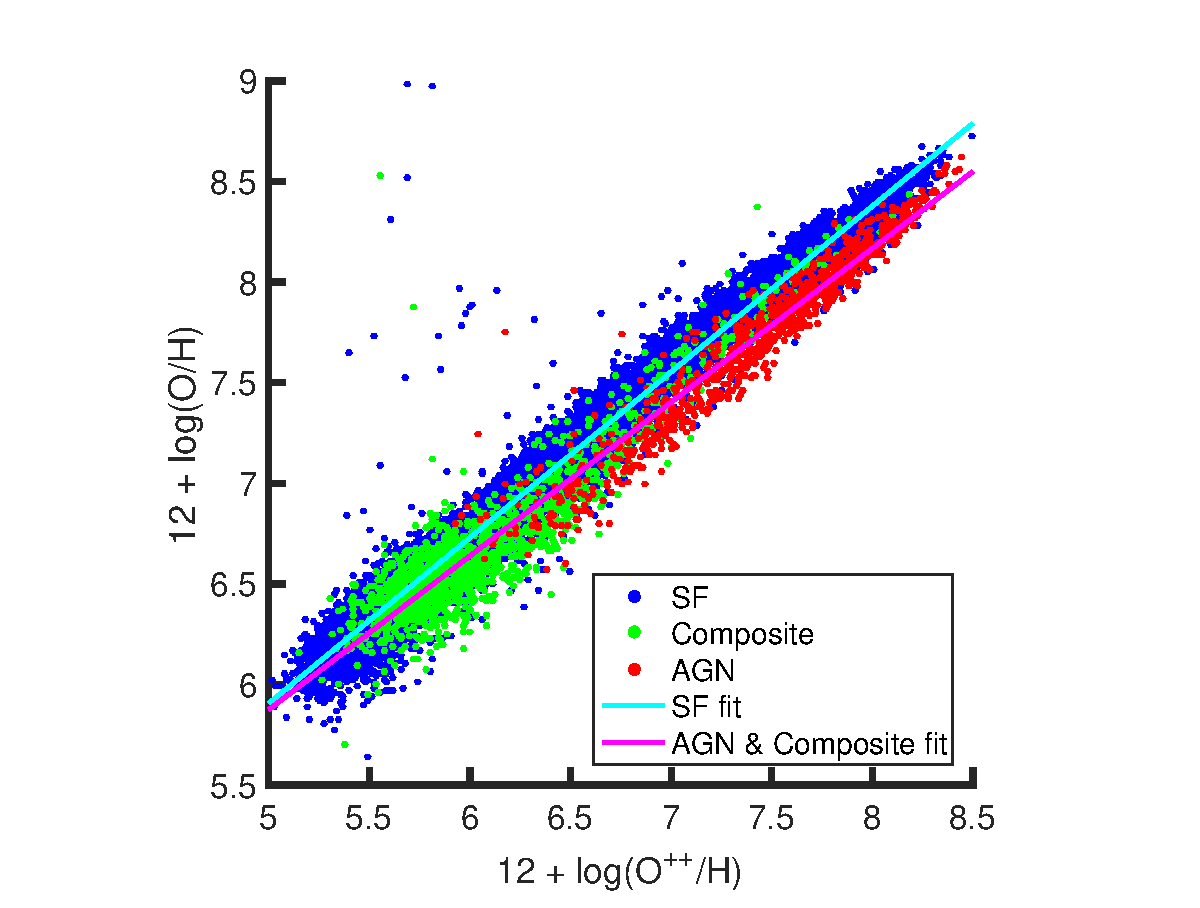
\includegraphics[width=0.75\textwidth]{Images/Paper3/Zlow_v_Zreal_1sig_I06_BPTclass_fits}
    \caption[O$^++$/H versus O/H]{$12 + \log{\text{O}^{++}/\text{H}}$ versus \OH 
    for those galaxies with $M_r > -20$ as calculated with the direct method; 
    the galaxies are colored by their classification in the BPT diagrams 
    \citep[from][]{Brinchmann04}.  Two linear models have been fit to three 
    groups in the sample: star-forming and AGN/composite galaxies; the best fit 
    parameters can be found in Table \ref{tab:ab}.}
    \label{fig:lowVreal}
\end{figure}

We derive an ICF for O$^+$ to overcome some limitations on the observations of 
dwarf galaxies in SDSS to bolster our sample size.  Because we are studying 
dwarf galaxies, the [\ion{O}{2}] $\lambda 3727$ doublet necessary for estimating 
the abundance of O$^+$ is only available for objects within the redshift range 
$0.02 < z < 0.03$ \citep[see Sec. \ref{sec:SDSS_limits_P3} and][for more 
details]{Douglass17a}.  To be able to study SDSS galaxies at redshifts less than 
0.02, we need to find an alternate way to estimate the abundance of O$^+$.  
Ordinarily, we would use an ICF to replace the missing ionization stage, as 
outlined in Sec. \ref{sec:DirectTe} for the nitrogen abundance.  Because the 
[\ion{O}{2}] $\lambda 3727$ emission line is normally available for analysis, 
there are no approximations available for the ICF for the amount of 
singly-ionized oxygen.  To construct an ICF appropriate for our dwarf galaxy 
sample, we compare \OH to $12 + \log{\text{O}^{++}/\text{H}}$ as calculated by 
the Direct $T_e$ method for all galaxies in SDSS with $M_r > -20$.  Recognizing 
that the relative amounts of singly- and doubly-ionized oxygen will depend on 
the hardness of a galaxy's spectrum, we use a Baldwin-Phillips-Terlevich (BPT) 
diagram \citep{Baldwin81} to classify each galaxy as star-forming, AGN, or 
composite (containing characteristics of both a star-forming region and an AGN).  
Noting a strong separation in the relationship between O$^{++}$/H and O/H with 
respect to the galaxies' BPT classifications by \cite{Brinchmann04}, we fit two 
linear models to the sample, seen in Fig. \ref{fig:lowVreal} and defined as 
\begin{equation}\label{eq:fit}
    12 + \log{\text{O}/\text{H}} = a(12 + \log{\text{O}^{++}/\text{H}}) + b
\end{equation}
The values for $a$ and $b$ for the two classes are listed in Table \ref{tab:ab}.



\begin{table}
\centering

    \begin{tabular}{l|c|c|c}
         & SF (dwarf) & SF ($M_r > -20$) & AGN \& Composite\\
        \hline
        $a$ & $0.84 \pm 0.013$ & $0.824 \pm 0.0010$ & $0.764 \pm 0.0035$\\
        $b$ & $1.61 \pm 0.094$ & $1.787 \pm 0.0065$ & $2.05 \pm 0.023$
    \end{tabular}
    
    \caption[Coefficients of oxygen abundance fits]{Coefficients for the linear 
    trends (Eqn. \ref{eq:fit}) fit to the SF galaxies (dwarf and those with 
    $M_r > -20$) and AGN and composite galaxies.  With these trends, we can now 
    calculate the total oxygen abundance for a galaxy with knowing only the 
    O$^{++}$/H abundance.}
    
    \label{tab:ab}
    
\end{table}



As expected, the star-forming galaxies have less doubly ionized oxygen than 
both the composite and AGN galaxies.  Since the degree of ionization depends on 
the temperature of the stars ionizing the gas, this means that the star-forming 
galaxies have cooler ionizing sources than the composite and AGN galaxies.

For those star-forming dwarf galaxies for which [\ion{O}{2}] $\lambda$3727 is 
not observed in the SDSS spectra, we use the coefficients for the star-forming 
dwarf galaxies with Eqn. \ref{eq:fit} to calculate the total oxygen abundance in 
the galaxy based on the amount of doubly-ionized oxygen found with Eqn. 4 of 
\cite{Douglass17a}.  While we list the coefficients for the linear models of 
both those galaxies with absolute magnitudes $-17 > M_r > -20$ and the AGN and 
composite galaxies in Table \ref{tab:ab}, we do not use them to calculate the 
chemical abundances of these galaxies for the reasons outlined in Section 
\ref{sec:DirectTe}.



%%%%%%%%%%%%%%%%%%%%%%%%%%%%%%%%%%%%%%%%%%%%%%%%%%%%%%%%%%%%%%%%%%%%%%%%%%%%%%%%
%
%    DATA
%
%%%%%%%%%%%%%%%%%%%%%%%%%%%%%%%%%%%%%%%%%%%%%%%%%%%%%%%%%%%%%%%%%%%%%%%%%%%%%%%%
\section[SDSS Data]{SDSS data and galaxy selection}

The SDSS Data Release 7 (DR7) \citep{Abazajian09} is a wide-field multiband 
imaging and spectroscopic survey employing a drift scanning technique to map 
approximately one-quarter of the northern sky.  Photometric data in the 
five-band SDSS system --- $u$, $g$, $r$, $i$, and $z$ --- are taken with a 
dedicated 2.5-meter telescope at the Apache Point Observatory in New Mexico 
\citep{Fukugita96, Gunn98}.  Follow-up spectroscopic analysis is performed on 
galaxies with a Petrosian $r$-band magnitude $m_r < 17.77$ \citep{Lupton01, 
Strauss02}.  The spectra are taken using two double fiber-fed spectrometers and 
fiber plug plates with a minimum fiber separation of 55"; the observed 
wavelength range is $3800\text{\AA}$ to $9200\text{\AA}$ with a resolution 
$\lambda / \Delta \lambda \sim$1800 \citep{Blanton03}.  We use emission-line 
flux data from the MPA-JHU value-added catalog\footnote{Available at 
\url{http://www.mpa-garching.mpg.de/SDSS/DR7/}}, which is based on the SDSS DR7 
sample of galaxies.  All flux values have been corrected for dust reddening with 
the \cite{Cardelli89} extinction curve as implemented in pyNeb 
\citep{Luridiana15}; we assume the theoretical ratio H$\alpha$/H$\beta = 2.86$ 
at 10,000 K and 100 cm$^{-3}$ \citep{Osterbrock89}.

We use the stellar mass estimates from the NASA-Sloan Atlas \citep{Blanton11}.  
The \ion{H}{1} mass estimates are from the 70\% complete ALFALFA catalog 
$\alpha.70$ \citep{Giovanelli05}; \ion{H}{1} detections were matched to the SDSS 
galaxies by locating the nearest optical counterpart identified in the 
$\alpha.70$ catalog within 1 arcmin.  Absolute magnitudes, colors, and all other 
additional data are from the KIAS value-added galaxy catalog 
\citep{Choi10,Blanton05}.  Galaxy colors are rest-frame colors which have been 
$K$-corrected to a redshift of 0.1; they are corrected for galactic extinction 
and calculated with model magnitudes.  All galaxies have been visually inspected 
to remove any galaxy fragments or duplicates.


%-------------------------------------------------------------------------------
\subsection{Spectroscopic selection}\label{sec:SDSS_limits_P3}

We employ the same requirements for our sample as in 
\cite{Douglass17a,Douglass17b}: all galaxies must have
\begin{enumerate}
    \item{$M_r > -17$ (dwarf galaxies);}
    \item{a minimum $5\sigma$ detection of H$\beta$;}
    \item{a minimum $1\sigma$ detection of [\ion{O}{3}] $\lambda 4363$;}
    \item{a flux $> 0$ for [\ion{O}{2}] $\lambda 3727$, [\ion{O}{3}] $\lambda \lambda 4959,5007$, and [\ion{N}{2}] $\lambda \lambda 6548,6584$;}
    \item{$T(\text{[\ion{O}{3}]}) > 3\times 10^4 \text{ K}$;}
    \item{a star-forming BPT classification by \cite{Brinchmann04}.}
\end{enumerate}

For those galaxies with a redshift $z \gtrsim 0.02$, we use the 
\texttt{oii\_flux} value from the MPA-JHU catalog in place of their [\ion{O}{2}] 
$\lambda \lambda 3726,3729$ flux measurement.  See \cite{Douglass17a} for 
further details on each of these requirements.


%-------------------------------------------------------------------------------
\subsection{Void classification}

The large-scale environment of the galaxies is determined using the void catalog 
compiled by \cite{Pan12}, which was constructed with the galaxies in SDSS DR7 
catalog.  The VoidFinder algorithm of \cite{Hoyle02} \citep[based on the 
algorithm described by][]{ElAd97} removes all isolated galaxies (defined as 
having the third nearest neighbor more than 7 \hMpc away) using only galaxies 
with absolute magnitudes $M_r < -20$.  After applying a grid to the remaining 
galaxies, spheres are grown from all cells containing no galaxies until it 
encounters four galaxies on its surface.  A sphere must have a minimum 10 \hMpc 
radius to be classified as a void (or part of one).  If two spheres overlap by 
more than 10\%, they are considered part of the same void.  See \cite{Hoyle02} 
for a more detailed description of the VoidFinder algorithm.  Those galaxies 
that fall within these void spheres are classified as voids.  Galaxies that lie 
outside the spheres are classified as wall galaxies.  Because we cannot identify 
any voids within 5 \hMpc of the edge of the survey, we classify these galaxies 
as ``Uncertain.''

Of the $\sim$800,000 galaxies with spectra available in SDSS DR7, 9519 are 
dwarf galaxies.  Applying the spectroscopic cuts, our sample includes 993 void 
dwarf galaxies and 759 wall dwarf galaxies.


%%%%%%%%%%%%%%%%%%%%%%%%%%%%%%%%%%%%%%%%%%%%%%%%%%%%%%%%%%%%%%%%%%%%%%%%%%%%%%%%
%
%    ANALYSIS & RESULTS
%
%%%%%%%%%%%%%%%%%%%%%%%%%%%%%%%%%%%%%%%%%%%%%%%%%%%%%%%%%%%%%%%%%%%%%%%%%%%%%%%%
\section[Analysis \& Results]{Abundance analysis and results}

Our primary objective is to perform a relative measurement of gas-phase 
abundances of dwarf galaxies to discern how their chemical evolution is affected 
by the large-scale environment.

All line ratios listed are ratios of the emission-line fluxes.  Galaxies with 
low metallicities have $Z =$ \OH $< 7.6$ \citep{Pustilnik06}; galaxies with high 
metallicities have $Z > 8.2$ \citep{Pilyugin06}.  The solar metallicity 
$Z_\odot = 8.86$ \citep{Delahaye06}.


%-------------------------------------------------------------------------------
\subsection{Estimation of uncertainties}

% Uncertainties
Uncertainties in the computed abundances are estimated using a Monte-Carlo 
method.  Using the measured line fluxes and scaled uncertainty estimates, we 
calculate 100,000 abundance estimates.  For each abundance estimate, a new 
positive ``fake'' line flux is drawn from a normal distribution.  We use the 
standard deviation in these sets of 100,000 calculated abundance values for the 
error in our abundance estimate.  See \cite{Douglass17a} for a more in-depth 
description of this process.


%-------------------------------------------------------------------------------
\subsection{Sources of systematic error}

Many physical properties of galaxies exhibit a radial dependence \citep{Bell00}.  
As a result, abundance estimates can depend on where the spectroscopic fiber is 
placed on the galaxy.  The estimated abundance will not necessarily be 
representative of a global abundance value if not all of the galaxy's light is 
contained within the fiber.  \cite{Belfiore17} show that both the metallicity 
and N/O ratio gradients are relatively flat for lower mass galaxies 
($\log(M/M_\odot) = 9$) and steepen with increasing stellar mass.  In SDSS DR7, 
the spectroscopic fiber diameter is 3"; this corresponds to a minimum physical 
diameter of 1.31 $h^{-1}$kpc at a redshift $z < 0.03$.  For most of the dwarf 
galaxies in this study, this contains the majority of their angular size.  
Assuming the abundance gradients remain flat for dwarf galaxies as suggested by 
the results of \cite{Belfiore17}, then our estimates of the gas-phase chemical 
abundances for our sample of dwarf galaxies are independent of the location of 
the spectral fiber on the galaxies' surfaces.

The selection criteria outlined in Section \ref{sec:SDSS_limits_P3} limit our 
sample to only star-forming dwarf galaxies.  As a result, this is not a 
representative sample of the entire dwarf galaxy population.  We are only able 
to discuss the influence of the large-scale environment on star-forming dwarf 
galaxies in this study.  Unfortunately, it is impossible to estimate the 
chemical abundances of red dwarf galaxies with the direct $T_e$ method because 
the UV photons from young stars are needed to excite the interstellar gas.


%-------------------------------------------------------------------------------
\subsection{Dwarf galaxy abundances}

% Results table (machine-readable)
\begin{sidewaystable}
\centering

\begin{tabular}{cccccccccccc}
Index\footnote{KIAS-VAGC galaxy index number} & R.A. & Decl. & Redshift & $M_r$ & \multicolumn{2}{c}{$12 + \log \left( \frac{\text{O}}{\text{H}} \right)$} & \multicolumn{2}{c}{$12 + \log \left( \frac{\text{N}}{\text{H}} \right)$} & \multicolumn{2}{c}{$\log \left( \frac{\text{N}}{\text{O}} \right)$} & Void/Wall \\
\hline \\
63713 & \RA{09}{20}{04}{.27} & -\dec{00}{30}{08}{.97} & 0.0257 & -16.73 & 7.80 & $\pm$0.41 & 6.83 & $\pm$0.28 & -0.97 & $\pm$0.49 & Wall \\
73537 & \RA{09}{25}{24}{.23} & +\dec{00}{12}{40}{.39} & 0.0250 & -16.94 & 7.94 & $\pm$0.34 & 6.76 & $\pm$0.24 & -1.18 & $\pm$0.41 & Wall \\
75442 & \RA{13}{13}{24}{.25} & +\dec{00}{15}{02}{.95} & 0.0264 & -16.81 & 7.55 & $\pm$0.35 & 6.73 & $\pm$0.24 & -0.82 & $\pm$0.42 & Void \\
168874 & \RA{11}{45}{13}{.16} & -\dec{01}{48}{17}{.68} & 0.0273 & -16.99 & 8.16 & $\pm$0.31 & 6.94 & $\pm$0.21 & -1.21 & $\pm$0.37 & Wall \\
184308 & \RA{09}{39}{09}{.38} & +\dec{00}{59}{04}{.15} & 0.0244 & -16.73 & 7.36 & $\pm$0.43 & 6.71 & $\pm$0.31 & -0.65 & $\pm$0.53 & Wall\\
\end{tabular}

\caption[Chemical abundances of subset of 135 dwarf galaxies]{Five of the 135 dwarf galaxies analyzed from SDSS DR7.  The flux values for all required emission lines can be found in the MPA-JHU value-added catalog.  Metallicity values are calculated using the direct $T_e$ method, with error estimates via a Monte Carlo method.  The void catalog of \cite{Pan12} is used to classify the galaxies as either Void or Wall.  If a galaxy is located too close to the boundary of the SDSS to identify whether or not it is inside a void, it is labeled as Uncertain.  (This table is available in its entirety in machine-readable form.)}

\label{tab:Results_P2}

\end{sidewaystable}


The abundances estimated using the direct $T_e$ method for our dwarf galaxy 
sample are listed in Table \ref{tab:Results_P3}.  Also included are other 
significant characteristics and identification for the galaxies, including their 
large-scale environmental classification.


\subsubsection{Oxygen and nitrogen abundances}

\begin{figure*}
    \centering
    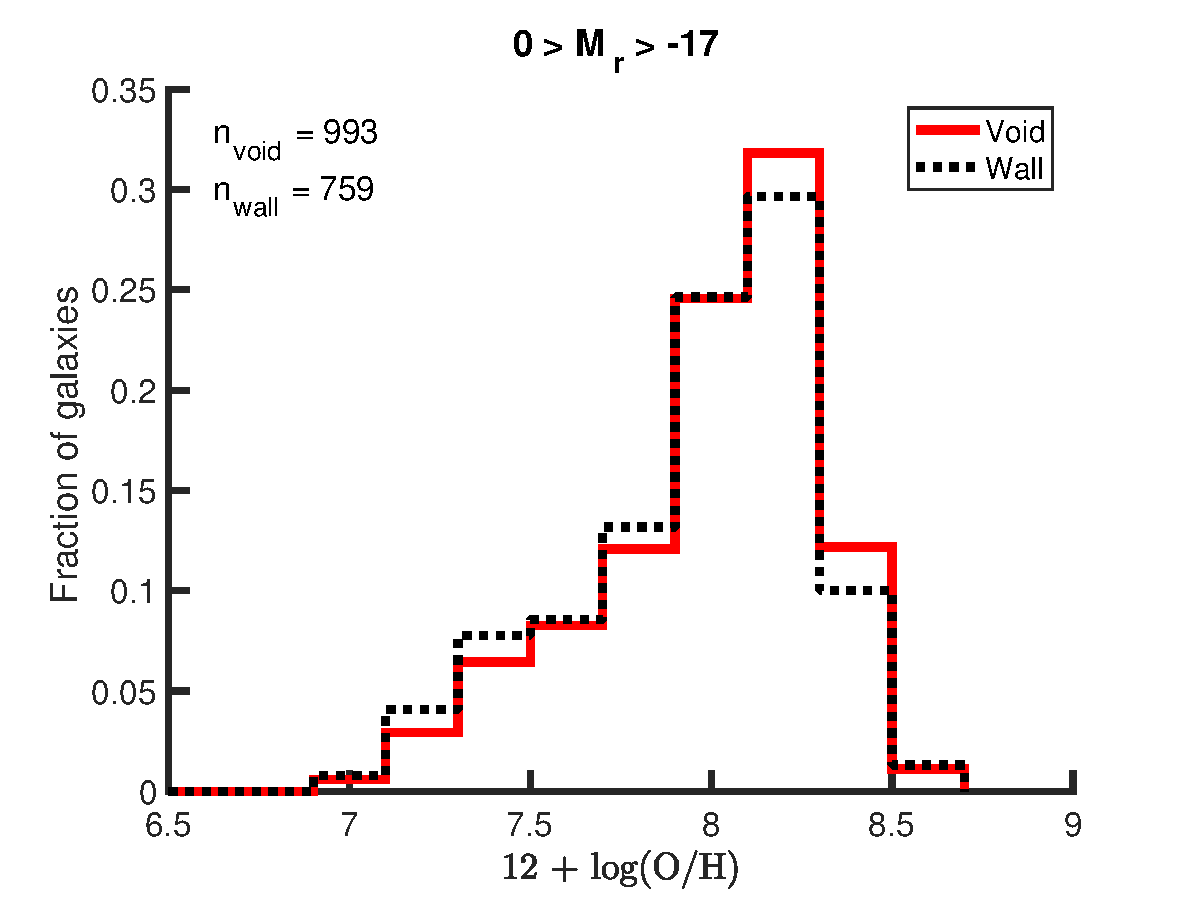
\includegraphics[width=0.49\textwidth]{Images/Paper3/1sig_dwarf_SF_t3_12logOHrelations_dust_hist}
    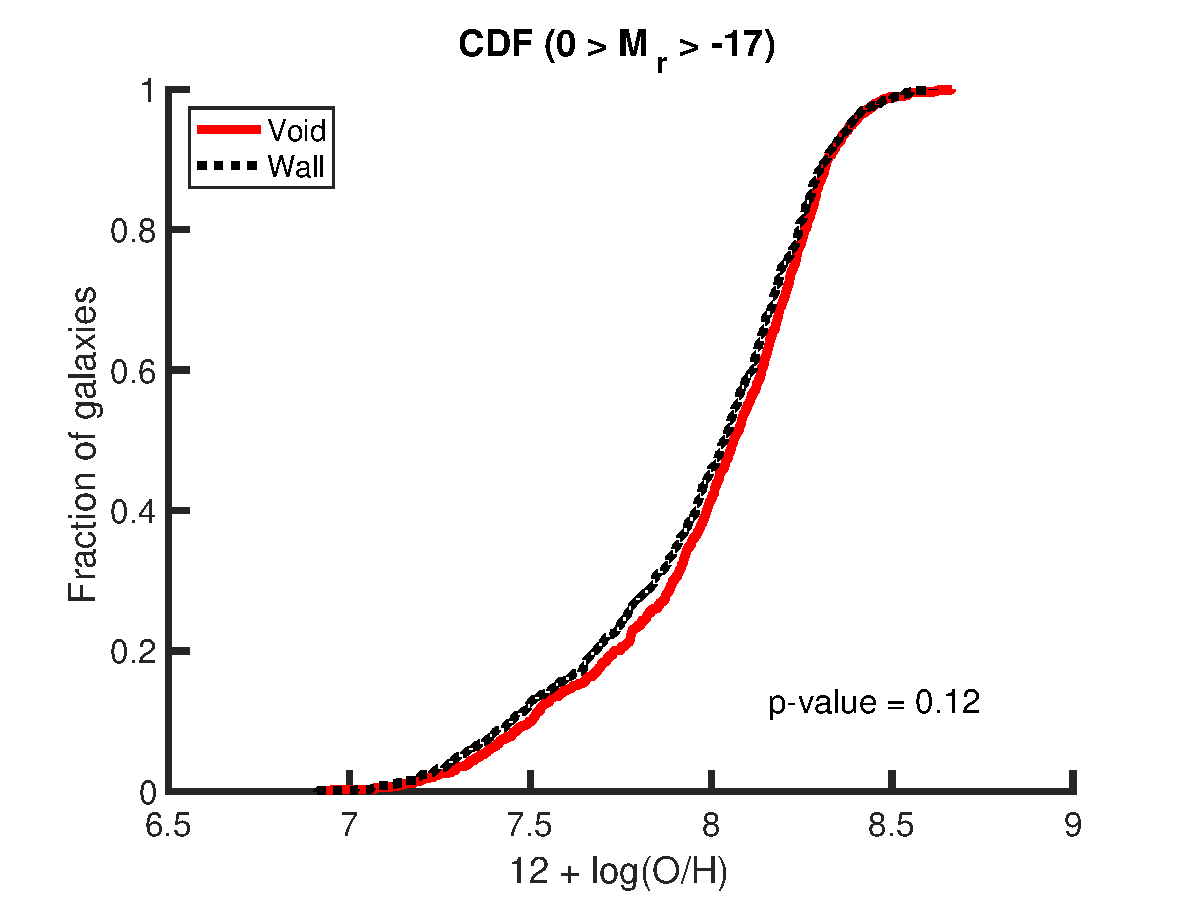
\includegraphics[width=0.49\textwidth]{Images/Paper3/1sig_dwarf_SF_t3_12logOHrelations_dust_CDF}
    \caption[O/H distribution for dwarf galaxy sample]{Gas-phase metallicity of 
    void dwarf (red solid line) and wall dwarf (black dashed line) galaxies.  A 
    two-sample K-S test of the two data sets results in an asymptotic $p$-value 
    of 0.12, indicating a 12\% probability that a test statistic greater than 
    the observed value of 0.06 will be seen if the void sample is drawn from the 
    wall sample.  This is reflected visually, as there appears to be a slight 
    but statistically significant significant large-scale environmental 
    influence on the metallicity of dwarf galaxies.}
    \label{fig:met1sig_P3}
\end{figure*}

\begin{figure*}
    \centering
    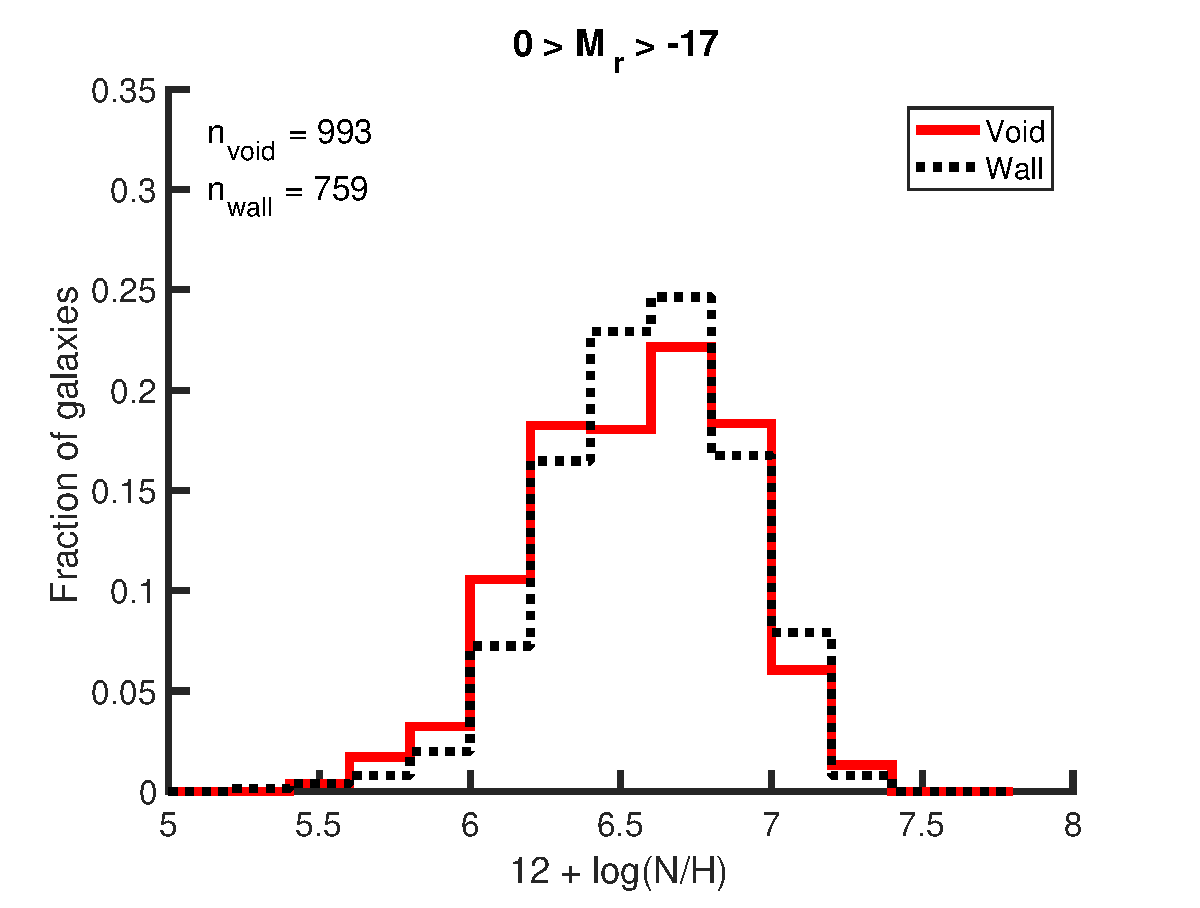
\includegraphics[width=0.49\textwidth]{Images/Paper3/1sig_dwarf_SF_t3_12logNHrelations_dust_hist}
    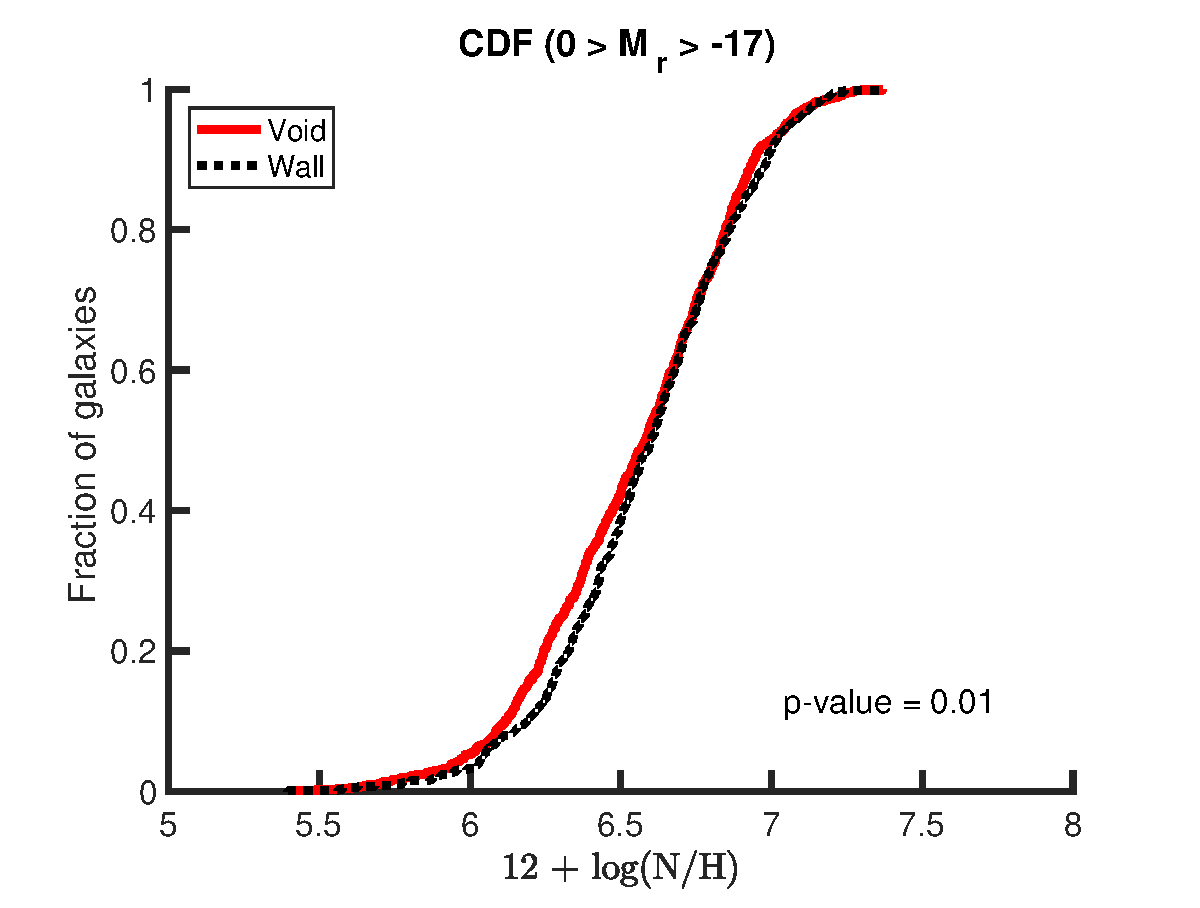
\includegraphics[width=0.49\textwidth]{Images/Paper3/1sig_dwarf_SF_t3_12logNHrelations_dust_CDF}
    \caption[N/H distribution for dwarf galaxy sample]{Abundance of nitrogen 
    relative to hydrogen of void dwarf (red solid line) and wall dwarf (black 
    dashed line) galaxies.  A two-sample K-S test of the two data sets results 
    in an asymptotic $p$-value of 0.015, indicating a 1.5\% probability that a 
    test statistic greater than the observed value of 0.08 will be seen, if the 
    void sample is drawn from the wall sample.  This is reflected visually, as 
    the void dwarf galaxies appear to have lower values of the N/H ratio than 
    the wall dwarf galaxies.  There is a large-scale environmental dependence of 
    the chemical evolution of dwarf galaxies.}
    \label{fig:N_1sig_P3}
\end{figure*}

The distributions of oxygen and nitrogen abundances for dwarf galaxies as a 
function of large-scale environment are shown in Figures \ref{fig:met1sig_P3} 
and \ref{fig:N_1sig_P3}, respectively.  Both histograms show a slight shift 
between voids and walls in the chemical abundances of dwarf galaxies.  A 
two-sample Kolmogorov-Smirnov (K-S) test quantifies this observation --- a test 
statistic of 0.06 for oxygen and 0.08 for nitrogen are produced, corresponding 
to a probability of 12\% and 1.5\%, respectively, that a test statistic greater 
than or equal that observed will be measured if the void sample were drawn from 
the wall sample.  The cumulative distribution function (CDF) for each of these 
elements can be seen on the right in Figures \ref{fig:met1sig_P3} and 
\ref{fig:N_1sig_P3}; they show that void dwarf galaxies have slightly higher 
oxygen abundances and slightly lower nitrogen abundances than dwarf galaxies in 
more dense regions.  The K-S test quantifies the visual interpretation of these 
figures that the distributions of oxygen and nitrogen abundances are slightly 
different for star-forming dwarf galaxies in voids and walls.

The average and median values of the dwarf galaxy abundances also indicate a 
shift as a result of the large-scale environment.  The average oxygen abundance 
for void dwarf galaxies is $7.99\pm 0.007$ and the median is 8.06, while the 
average oxygen abundance for wall dwarf galaxies is $7.96\pm 0.009$ with a 
median value of 8.04.  This implies that the void dwarf galaxies have higher 
oxygen abundances by about 7\% (average shift of $0.03\pm 0.012$; median shift 
of 0.03) relative to wall dwarf galaxies.  In contrast, the average nitrogen 
abundance for void dwarf galaxies is only $6.55\pm 0.007$ with a median of 6.58, 
while the wall dwarf galaxies have an average nitrogen abundance of 
$6.58\pm 0.008$ and a median of 6.60.  The void dwarf galaxies have lower 
nitrogen abundances by about 10\% (an average shift of $0.04\pm 0.011$ and a 
median shift of 0.02) relative to wall dwarf galaxies.  A tabular version of 
this analysis can be found in Table \ref{tab:stats_p3}.


\subsubsection{Ratio of nitrogen to oxygen}

\begin{figure*}
    \centering
    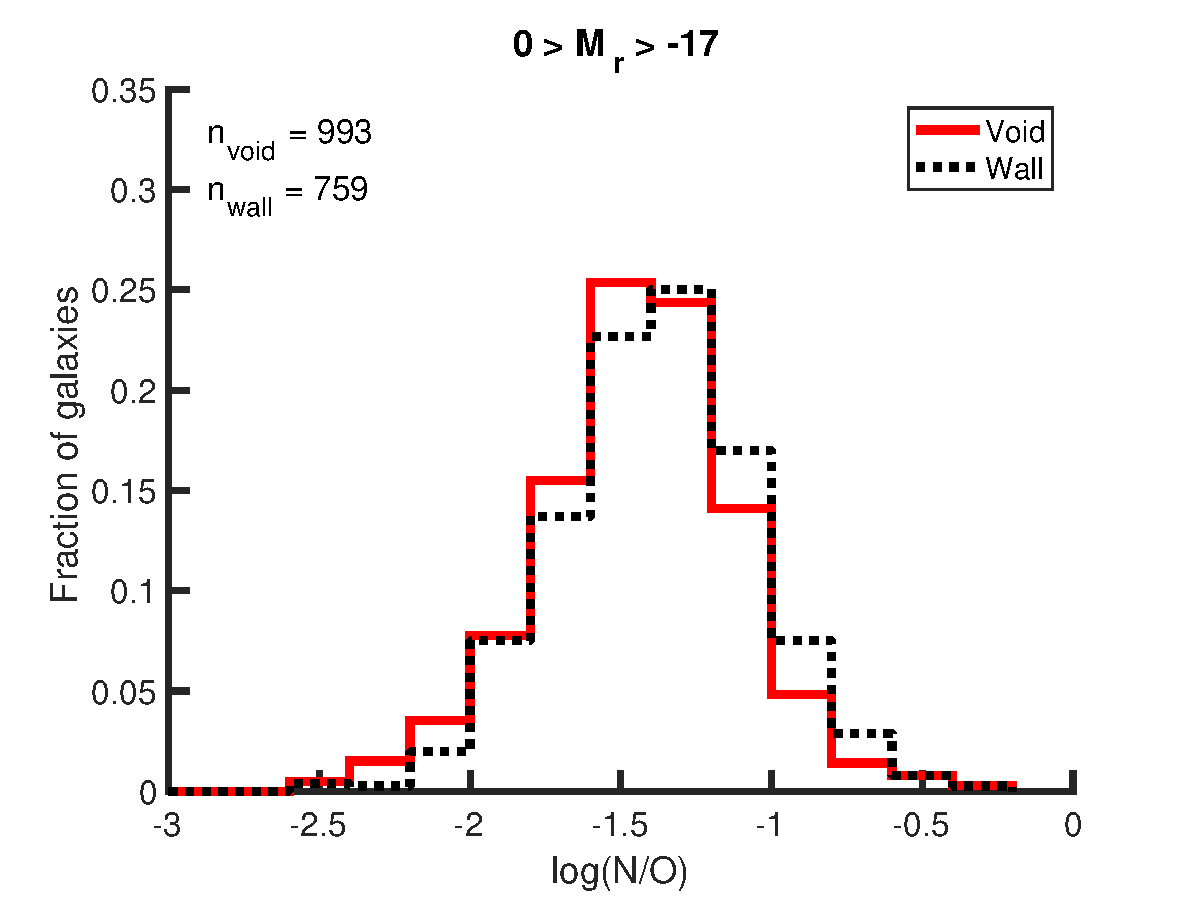
\includegraphics[width=0.49\textwidth]{Images/Paper3/1sig_dwarf_SF_t3_logNOrelations_dust_hist}
    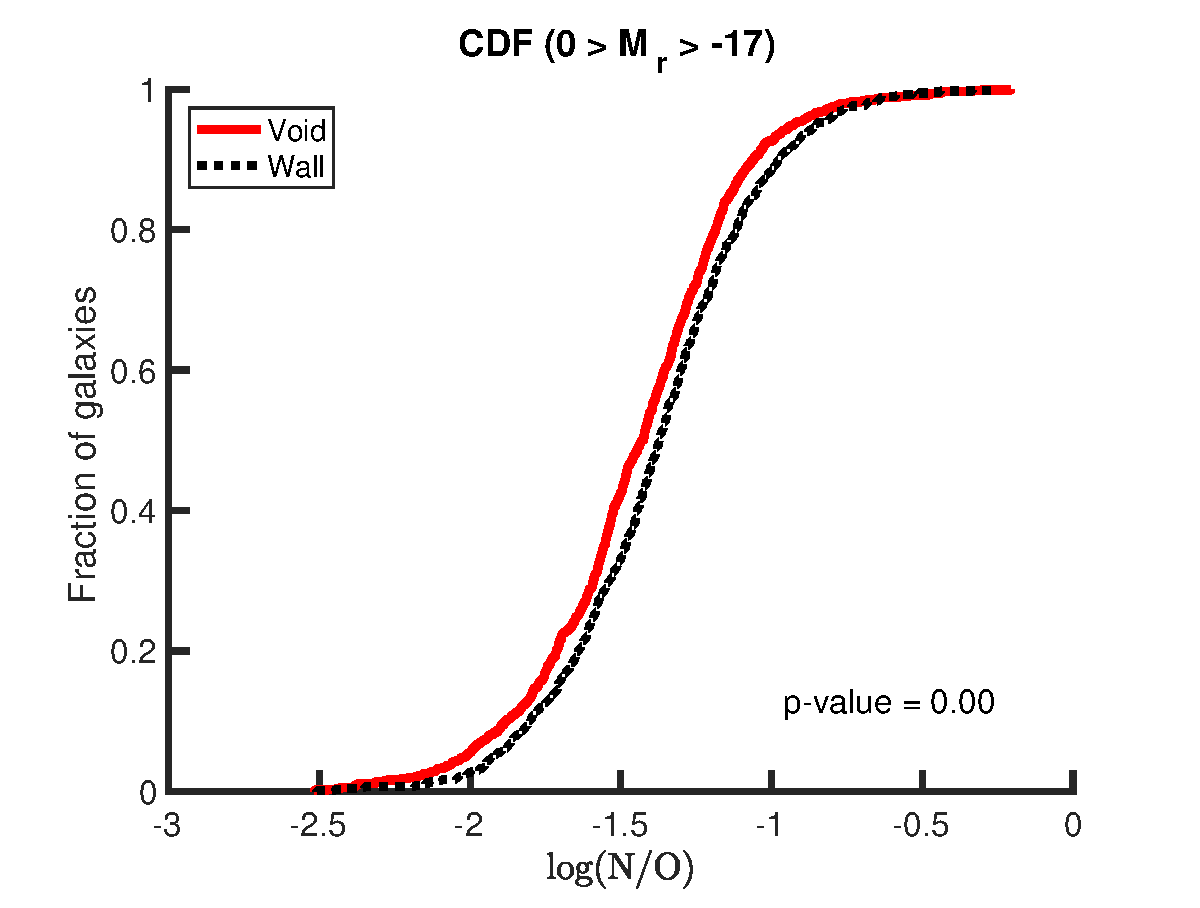
\includegraphics[width=0.49\textwidth]{Images/Paper3/1sig_dwarf_SF_t3_logNOrelations_dust_CDF}
    \caption[N/O distribution of dwarf galaxy sample]{Ratio of nitrogen to 
    oxygen of void dwarf (red solid line) and wall dwarf (black dashed line) 
    galaxies.  A two-sample K-S test of the two data sets results in an 
    asymptotic $p$-value of $2.6\times 10^{-4}$, indicating only a 0.03\% 
    probability that a test statistic greater than the observed value of 0.10 
    will be seen.  This is reflected visually, as there is a shift in the N/O 
    ratio between the two populations of dwarf galaxies --- the void galaxies 
    have a lower value of N/O than the wall galaxies.  There is a large-scale 
    influence on the relative chemical abundances of dwarf galaxies.}
    \label{fig:NOratio_P3}
\end{figure*}

The ratio of nitrogen to oxygen is also important to investigate, as it 
communicates the nucleosynthesis history of the galaxies.  As seen in Fig. 
\ref{fig:NOratio_P3}, the N/O abundance ratio also indicates a large-scale 
environmental influence on the chemical evolution of dwarf galaxies --- void 
dwarf galaxies have lower N/O ratios than dwarf galaxies in denser regions.  
This difference is quantified in the K-S test: the test returned a probability of 
only 0.03\% that a test statistic greater than or equal to 0.10 will be measured 
if the void sample was drawn from the wall sample.  The distribution of N/O 
abundance ratios for void dwarf galaxies is lower by about 17\% (an average 
shift of $0.07\pm 0.016$ and a median shift of 0.06) relative to the 
distribution of N/O ratios in wall dwarf galaxies.


% Statistics table
\begin{table}
    \centering
    
    \begin{tabular}{ccccccc}
        Environment & Average & Median & Average Shift\footnote{Wall -- Void (Positive shifts indicate that the wall values are greater than the void values; negative shifts indicate that the void values are greater than the wall values.)\label{fnote_P3}} & Median Shift\textsuperscript{\ref{fnote_P3}} & $p$-value & K-S Test Statistic\\
        \hline
        % Oxygen %%%%%%%%%%%%%%%%%%%%%%%%%%%%%%%%%%%%%%%%%%%%%%%%%%%%%%%%%%%%%%%
        \hline
        \multicolumn{7}{c}{\OH}\\
        \hline
        Void & $7.99\pm 0.007$ & 8.06 & \multirow{2}{*}{$-0.03\pm 0.012$} & \multirow{2}{*}{-0.03} & \multirow{2}{*}{0.1197} & \multirow{2}{*}{0.0569}\\
        Wall & $7.96\pm 0.009$ & 8.04 & & & & \\
        % Nitrogen %%%%%%%%%%%%%%%%%%%%%%%%%%%%%%%%%%%%%%%%%%%%%%%%%%%%%%%%%%%%
        \hline
        \multicolumn{7}{c}{\NH}\\
        \hline
        Void & $6.55\pm 0.007$ & 6.58 & \multirow{2}{*}{$0.04\pm 0.011$} & \multirow{2}{*}{0.02} & \multirow{2}{*}{0.0149} & \multirow{2}{*}{0.0750}\\
        Wall & $6.58\pm 0.008$ & 6.60 & & & & \\
        % N/O %%%%%%%%%%%%%%%%%%%%%%%%%%%%%%%%%%%%%%%%%%%%%%%%%%%%%%%%%%%%%%%%%
        \hline
        \multicolumn{7}{c}{\NO}\\
        \hline
        Void & $-1.45\pm 0.010$ & -1.43 & \multirow{2}{*}{$0.07\pm 0.016$} & \multirow{2}{*}{0.06} & \multirow{2}{*}{0.0003} & \multirow{2}{*}{0.1013}\\
        Wall & $-1.38\pm 0.012$ & -1.37 & & & & \\
    \end{tabular}
    
    \caption[Abundance statistics]{Statistics on the gas-phase oxygen, nitrogen, 
    and nitrogen relative to oxygen abundances in dwarf void and wall galaxies.  
    Combined with the histograms in Figures 
    \ref{fig:met1sig_P3}--\ref{fig:NOratio_P3}, these results indicate an 
    influence on the chemical evolution of galaxies by the large-scale 
    environment, especially on the relative abundance of nitrogen to oxygen.  
    Void galaxies have slightly higher oxygen and nitrogen abundances than wall 
    galaxies, but void galaxies have slightly lower N/O ratios than wall 
    galaxies.}
    
    \label{tab:stats_p3}
    
\end{table}


%-------------------------------------------------------------------------------
\subsection{Comparison to previously published oxygen abundance estimates}
% Compare to Tremonti et al. (2004)

\begin{figure}
    \centering
    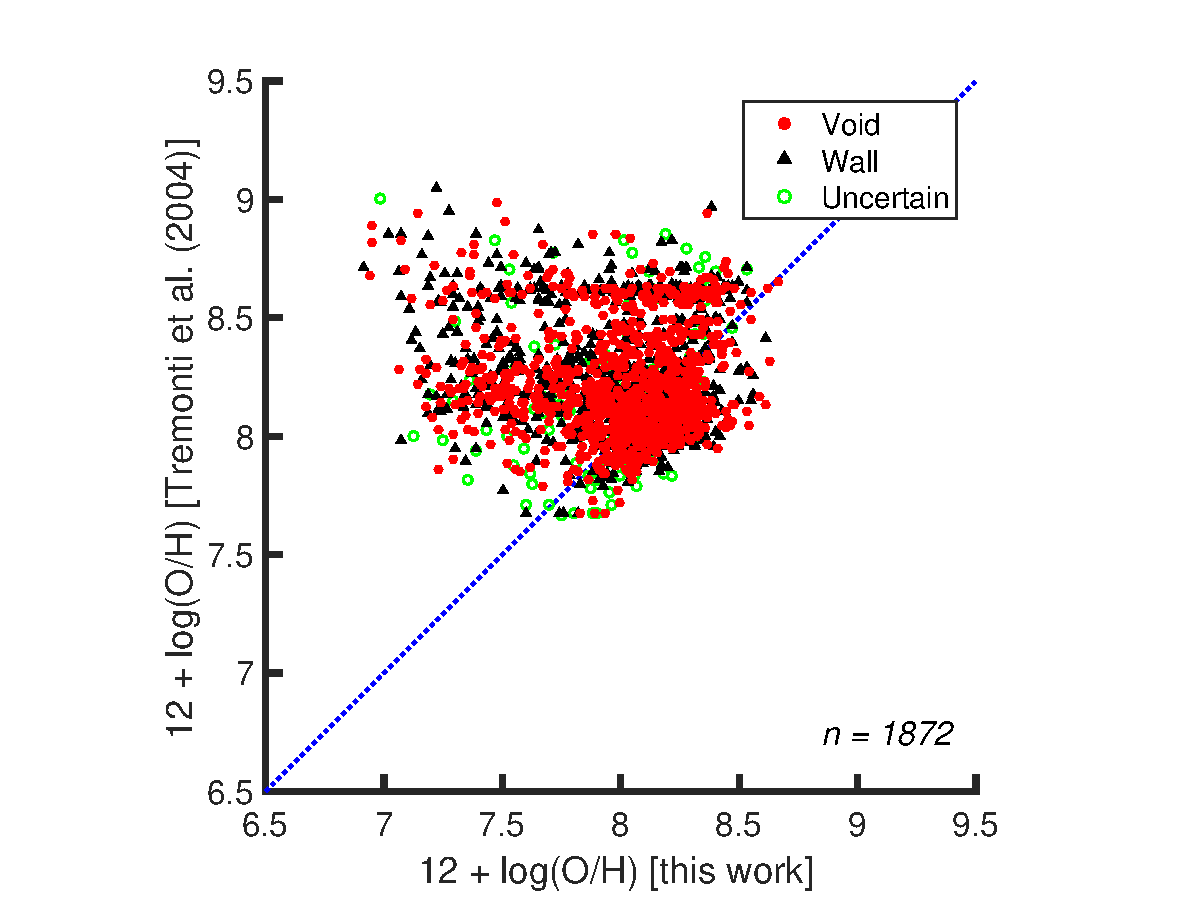
\includegraphics[width=0.75\textwidth]{Images/Paper3/1sig_dwarf_I06relations_SF_t3_T04comparison_dust}
    \caption[Comparison of O$^+$ approximation metallicities to 
    \cite{Tremonti04}]{Oxygen abundance comparison between our calculated 
    estimates with the O$^+$ approximation and those made by \cite{Tremonti04}.  
    Error bars have been omitted for clarity.  While the majority of our 
    abundance estimates agree reasonably well with the values already published, 
    it is clear that our estimates are often lower than the previously published 
    values.  It is well known that the strong-line methods \citep[like those 
    used by][]{Tremonti04} overestimate the oxygen abundance by as much as 0.3 
    dex \citep{Kennicutt03}.  Therefore, it is not surprising that the oxygen 
    abundances measured using the direct $T_e$ method are lower, particularly at 
    very low metallicities.}
    \label{fig:T04_comp}
\end{figure}

While no estimates of the nitrogen or N/O abundances have been made on a large 
selection of the SDSS galaxies, we can compare our oxygen abundance estimates to 
the metallicity values measured by \cite{Tremonti04}.  While we both use data 
from the MPA-JHU value-added catalog, \cite{Tremonti04} employs an empirical 
method to calculate the metallicity that is based on calibrated relationships 
between direct $T_e$ methods and strong-line ratios.  The results of this 
comparison are shown in Fig. \ref{fig:T04_comp}.  While the majority of our 
abundance estimates agree reasonably well with the values calculated by 
\cite{Tremonti04}, it is also clear that our estimates often predict abundances 
lower than those previously published.  This is especially true for the low 
metallicity regime ($12 + \log \left(\text{O}/\text{H}\right) < 7.6$).  Methods 
which are based on calibrations rarely use low metallicity galaxies in their 
source for calibrating.  As a result, empirical methods will often overestimate 
the abundance values, especially in the low-metallicity regime.  
\cite{Kennicutt03} show that strong-line methods (methods which make extreme use 
of the strong emission lines) can overestimate the metallicity abundances by as 
much as 0.3 dex.  Therefore, we are not surprised at the apparent lack of 
correlation between our oxygen abundance estimates and those of 
\cite{Tremonti04}.


%-------------------------------------------------------------------------------
\subsection{N/O versus O/H} \label{sec:NO_OH}

\begin{figure}
    \centering
    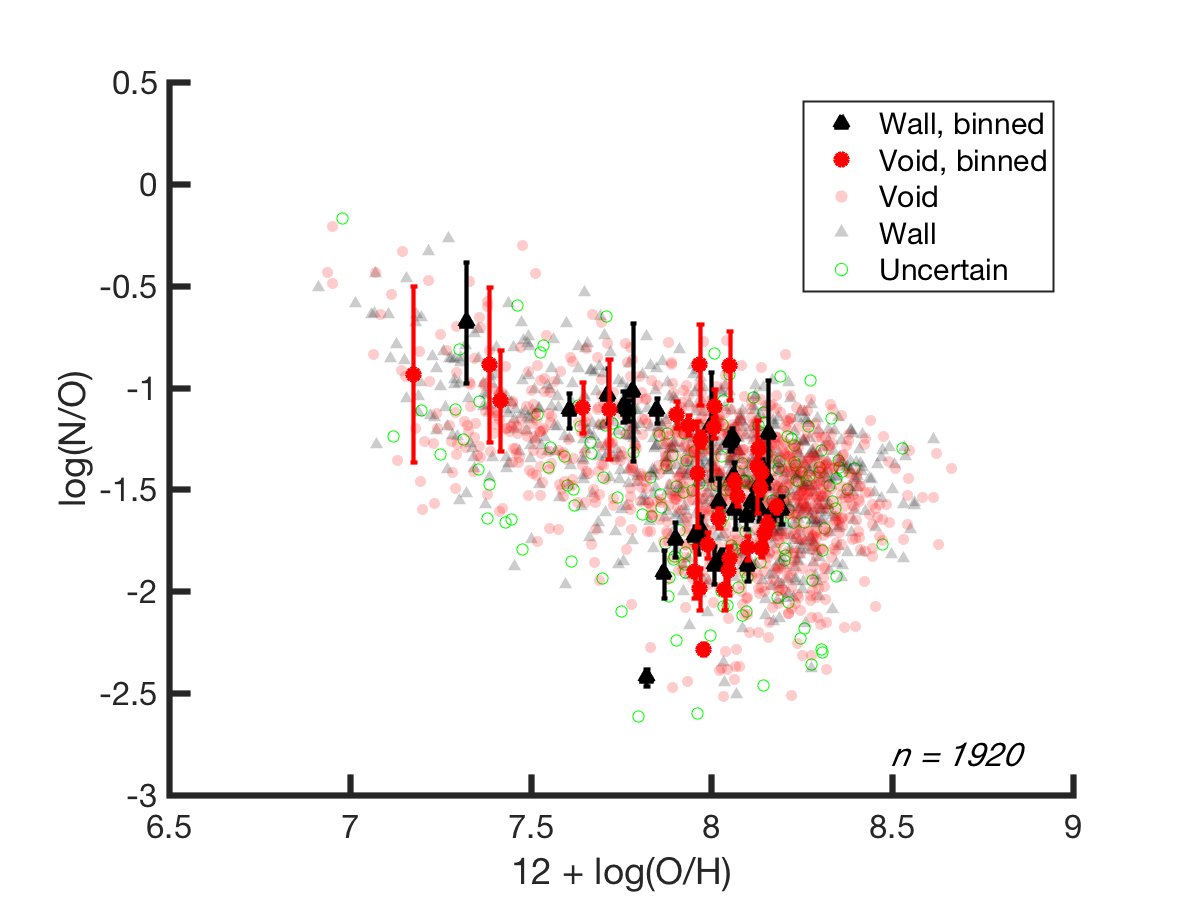
\includegraphics[width=0.75\textwidth]{Images/Paper3/1sig_I06relations_dwarf_SF_t3_dust_NSA_Z12logOH_logNO_scatterMbin}
    \caption[O/H versus N/O for star-forming dwarf galaxies]{Oxygen abundance 
    (\OH) versus the N/O ratio (\NO) for the dwarf galaxies in this study; the 
    average values of the galaxies' abundances when binned by stellar mass in 
    bins of width 0.1 are also shown.  As seen in \cite{Andrews13} and 
    \cite{Douglass17b}, while most of the mass bins are scattered together 
    around \NO $\sim$-1.5, there is a negative correlation between these two 
    abundance ratios.  There is no evidence of secondary nitrogen production in 
    this sample of star-forming dwarf galaxies, which would manifest as a 
    positive relationship between O/H and N/O at high metallicities.}
    \label{fig:NOvOH}
\end{figure}

Studying how the N/O ratio depends on the metallicity (gas-phase oxygen 
abundance) probes the nucleosynthetic production of nitrogen in stars within the 
galaxies.  It is believed that nitrogen can be produced as both a primary and 
secondary element, depending on the initial metallicity of the stars.  If there 
are enough of the heavy elements available when the stars are created (oxygen, 
carbon, etc.), then the CNO cycle can commence much earlier in the star's 
lifetime, resulting in a higher production of nitrogen than if the star is 
originally created with very few heavy elements.  If this is the case, then we 
should see no relationship between the N/O ratio and the oxygen abundance below 
a certain metallicity value (the primary nitrogen production phase); above this 
threshold metallicity, the N/O value should increase linearly with the oxygen 
abundance (the secondary nitrogen production phase).

As we see in Fig. \ref{fig:NOvOH}, there is no evidence of a secondary nitrogen 
production phase in our sample of dwarf galaxies.  This is in contrast with the 
evidence of secondary nitrogen production seen in Fig. \ref{fig:M_NO} of Sec. 
\ref{sec:Mass}; the source of this discrepancy is unclear.  The relationship 
between metallicity and the N/O ratio instead shows a large scatter with no 
clear correlation between the N/O ratio and the oxygen abundance at metallicity 
values higher than $\sim$7.9.  Below this value, we actually observe a negative 
correlation between the N/O ratio and the oxygen abundance.  This would indicate 
a constant value of nitrogen being synthesized in the galaxies independent of 
the amount of oxygen being produced.  A negative correlation similar to this was 
also observed by \cite{Andrews13} and \cite{Douglass17b}.   \cite{Andrews13} 
note that they measure a slope of -0.21 for their stellar mass-binned galaxies 
with metallicities \OH $< 8.5$, while \cite{Douglass17b} finds a slope of 
$-0.38\pm 0.078$ for dwarf galaxies.  A linear fit to our dwarf galaxy sample 
has a slope of $-0.52\pm 0.041$, steeper than any previously measured.

\begin{figure}
    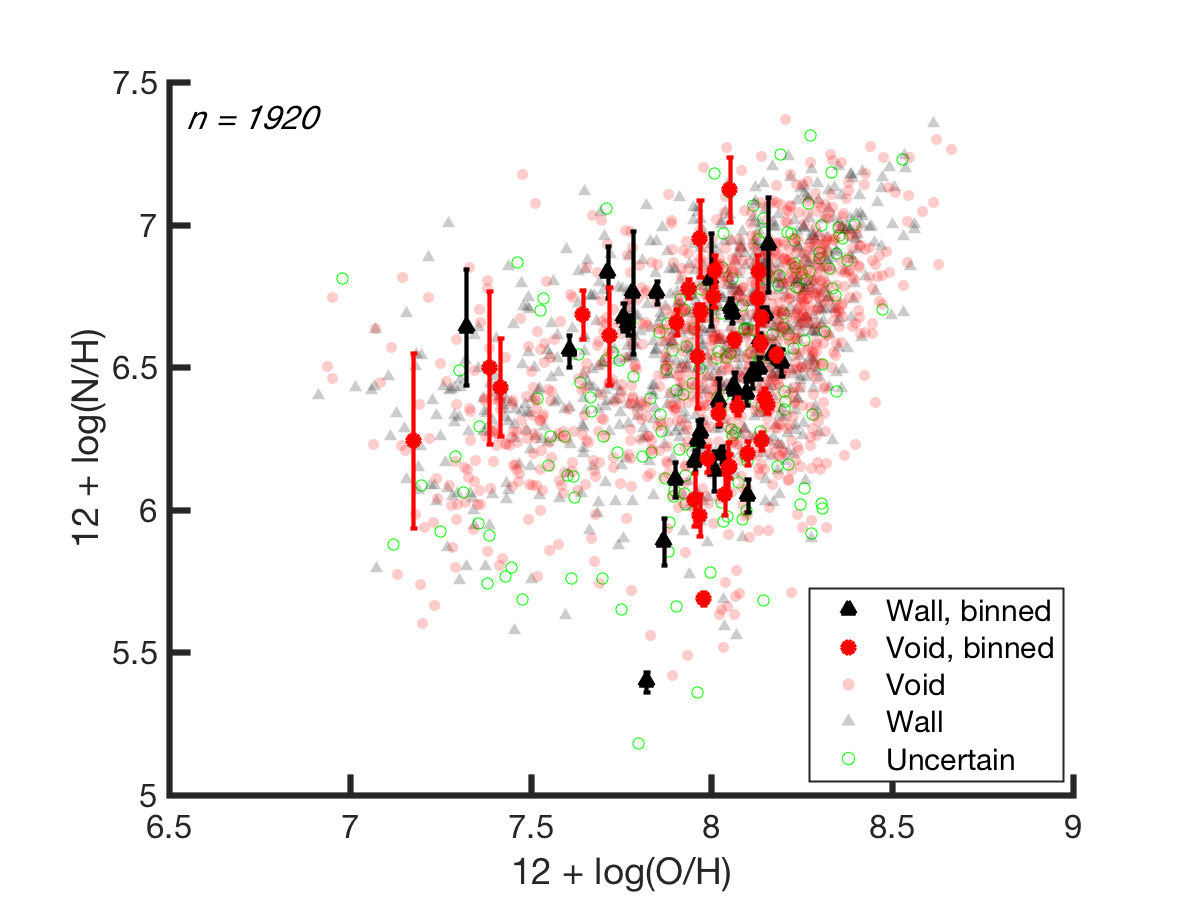
\includegraphics[width=0.75\textwidth]{Images/Paper3/1sig_I06relations_dwarf_SF_t3_dust_NSA_Z12logOH_N12logNH_scatterMbin}
    \caption[O/H versus N/H for star-forming dwarf galaxies]{Oxygen abundance 
    (\OH) versus nitrogen abundance (\NH) for the dwarf galaxies in this study; 
    the average values of the galaxies' abundances when binned by their stellar 
    mass in bins of width 0.1 are also shown.  There is evidence of two 
    evolutionary tracks for the star-forming dwarf galaxies here, one with a 
    much steeper slope than the other.}
    \label{fig:OvN_P3}
\end{figure}

Similar evidence of the nitrogen production phases can also be observed when 
looking at the relationship between the nitrogen and oxygen abundances relative 
to hydrogen.  Fig. \ref{fig:OvN_P3} depicts a negative relationship between the 
nitrogen and oxygen abundances.  A linear fit to the dwarf galaxies results in a 
slope of $0.48\pm 0.041$, less than the slope of $0.62\pm 0.078$ found by 
\cite{Douglass17b}.  These slopes both indicate that nitrogen is produced at a 
slower rate than oxygen in dwarf galaxies.  A nitrogen plateau in Fig. 
\ref{fig:NOvOH} would manifest itself as a relationship between the N/H and O/H 
ratios (shown in Fig. \ref{fig:OvN_P3}) with a linear slope of 1.  Secondary 
nitrogen production, a positive relationship in Fig. \ref{fig:NOvOH}, would 
correspond to a relationship between N/H and O/H in Fig. \ref{fig:OvN_P3} with a 
slope greater than 1.  If we split the dwarf galaxies into two populations based 
on their metallicity, we find that dwarf galaxies with extremely low 
metallicities (\OH $\leq 7.6$) have a slope of $-1.0\pm 0.21$ in Fig. 
\ref{fig:NOvOH} and $-0.0\pm 0.21$ in Fig. \ref{fig:OvN_P3}, while the dwarf 
galaxies with metallicities \OH $> 7.6$ have a slope of $-0.41\pm 0.069$ for O/H 
v. N/O and $0.59\pm 0.069$ for O/H v. N/H.  These slopes indicate that the 
production of nitrogen is independent of the oxygen abundance in systems with 
low metallicities, supporting the results found in \cite{Douglass17b}.

Fig. \ref{fig:OvN_P3} shows possible evidence for two evolutionary tracks for 
star-forming dwarf galaxies, irrespective of the large-scale environment.  The 
dwarf galaxies with extremely low metallicities appear to have less of a 
correlation between their oxygen and nitrogen abundances than those dwarf 
galaxies with higher metallicities.  The two tracks appear to merge between 
metallicity values $8 < 12 + \log(\text{O}/\text{H}) < 8.5$.  Those galaxies 
which have a much weaker relationship between their oxygen and nitrogen 
abundances correspond to those galaxies in Fig. \ref{fig:NOvOH} with a negative 
relationship between their N/O ratio and metallicity.  Further study is needed 
to understand why these galaxies have a different relationship between their 
oxygen and nitrogen abundances.

In both Figs. \ref{fig:NOvOH} and \ref{fig:OvN_P3}, there is no difference in 
the abundance ratio relationships between void dwarf galaxies and dwarf galaxies 
in denser regions.  The large-scale environment does not appear to influence the 
nucleosynthesis of nitrogen in dwarf galaxies.


%-------------------------------------------------------------------------------
\subsection{Stellar mass-abundance relations}\label{sec:Mass}

\begin{figure*}
    \centering
    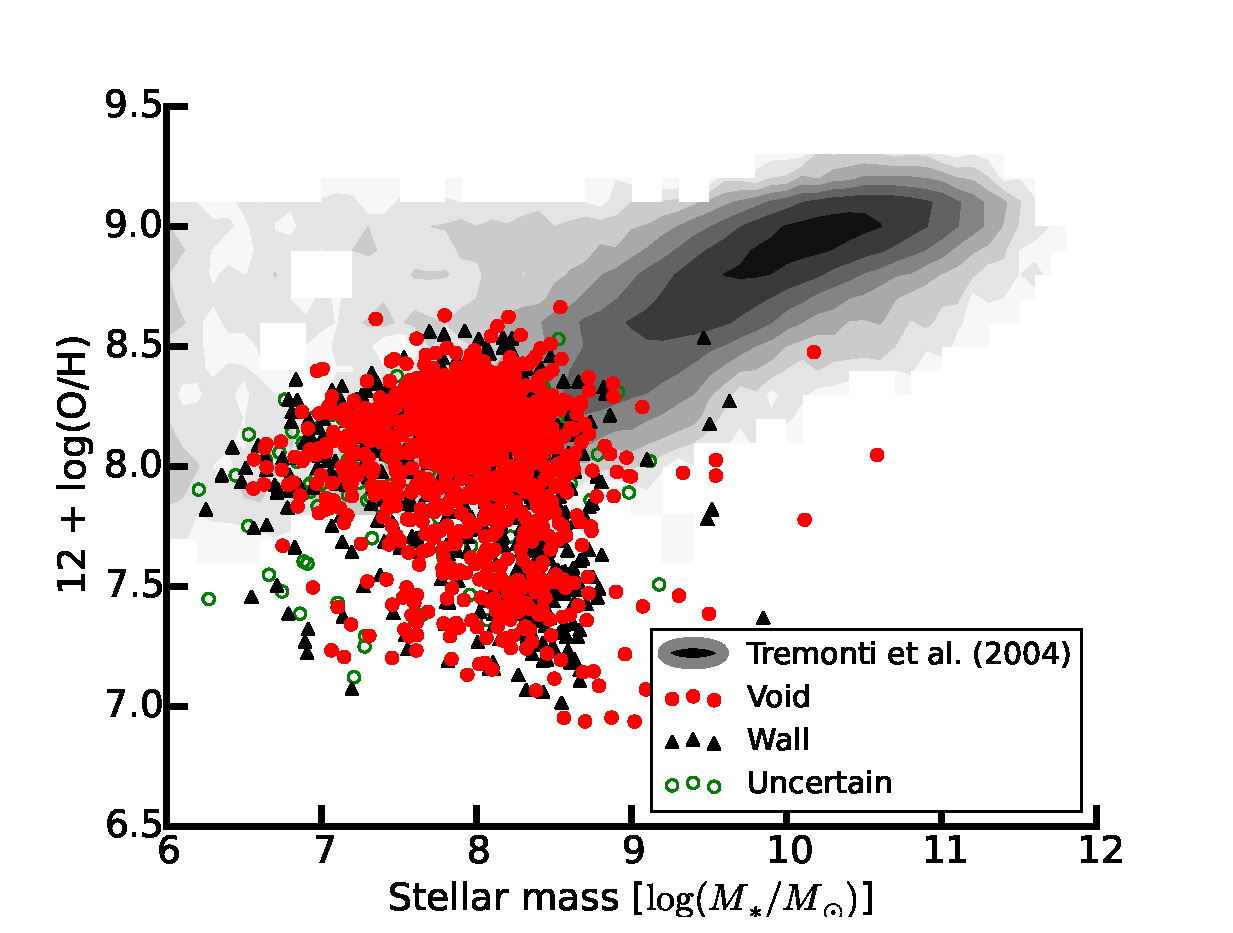
\includegraphics[width=0.49\textwidth]{Images/Paper3/MZ_1sig_I06relations_dwarf_SF_t3_dust_NSA_python}
    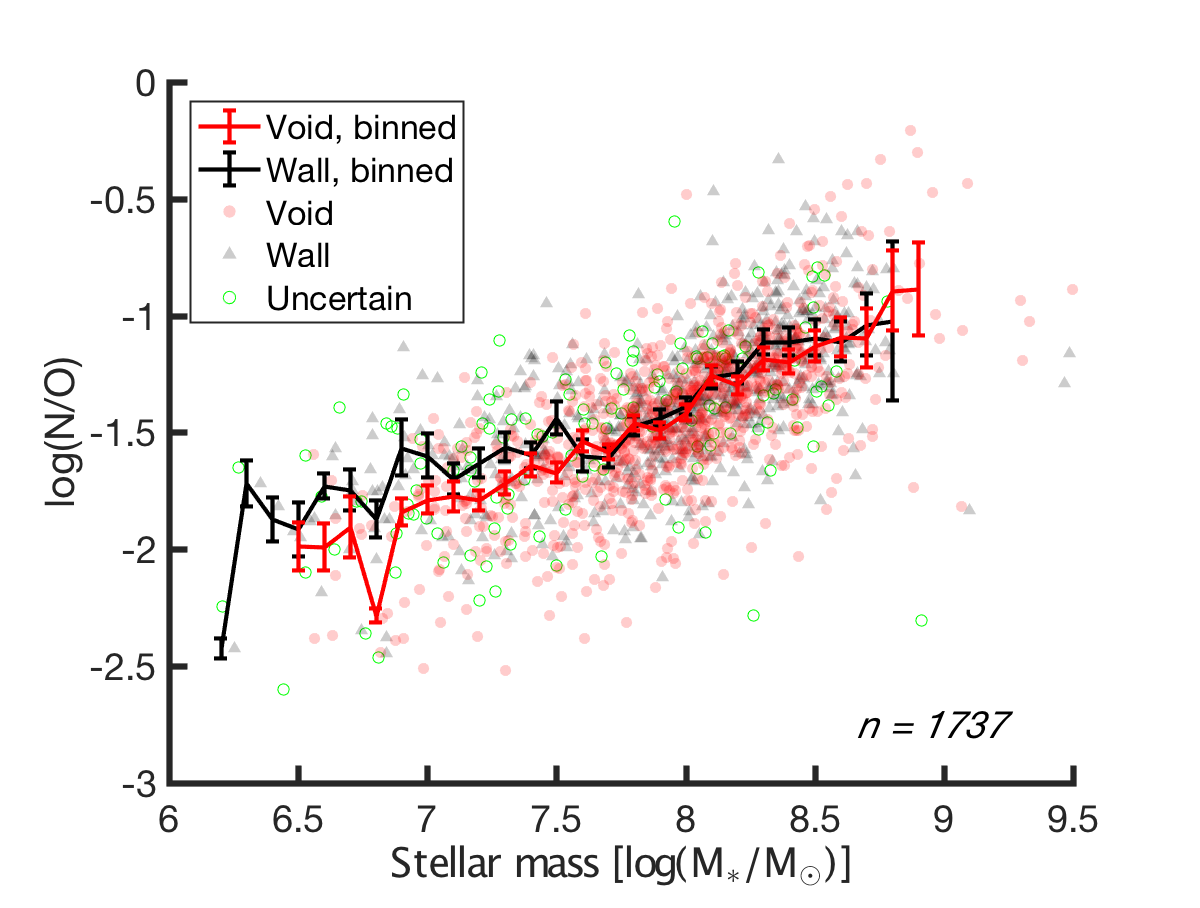
\includegraphics[width=0.49\textwidth]{Images/Paper3/MNO_1sig_I06relations_dwarf_SF_t3_dust_NSA_scatterMbin}
    \caption[$M_*$ versus N/O for star-forming dwarf galaxies]{Stellar mass 
    versus oxygen abundance (left panel) and N/O ratio (right panel).  We 
    include the metallicity results of \cite{Tremonti04} on the left to place 
    our dwarf galaxy abundance results in context.  On the right, we show the 
    average N/O values for the dwarf galaxies binned by stellar mass plotted 
    over the individual galaxies.  While most of our dwarf galaxies follow the 
    same trend as already seen in \cite{Tremonti04}, we note the existence of a 
    number of dwarf galaxies with much lower oxygen abundance values than what 
    would be predicted based on their stellar mass and the mass-metallicity 
    relation.  There is no clear difference between void and wall dwarf galaxies 
    in the mass-metallicity relation.  In the right-hand panel, though, we see 
    that the turn-off for the N/O plateau occurs at different masses for the two 
    large-scale environments.}
    \label{fig:M_NO}
\end{figure*}

Expanding on the mass-metallicity relation investigated in \cite{Douglass17a}, 
we look at the correlation between stellar mass and the oxygen abundance in our 
now substantially-larger sample of dwarf galaxies.  The mass-metallicity 
relation for our dwarf galaxies can be seen in Fig. \ref{fig:M_NO}.  We also 
include those galaxies from the MPA-JHU catalog with metallicity estimates from 
\cite{Tremonti04} to place our sample in context.  While most of our dwarf 
galaxies follow the same trend seen in \cite{Tremonti04}, we note the existence 
of a number of dwarf galaxies with much lower oxygen abundances than what would 
be predicted based on their stellar mass and the mass-metallicity relation.  
There is no discernible influence from the large-scale environment on the 
mass-metallicity relation for dwarf galaxies.

We also look at the N/O ratio as a function of stellar mass (Fig. 
\ref{fig:M_NO}, right panel).  Similar to the O/H--N/O relation studied in Sec. 
\ref{sec:NO_OH}, the N/O ratio is predicted to be constant below some critical 
mass; above this, the N/O ratio should increase linearly with the stellar mass.  
Unlike the relation seen in Fig. \ref{fig:NOvOH}, we see both the N/O plateau 
and the positive correlation on the right in Fig. \ref{fig:M_NO}.  To make the 
plot more readable, we also bin the galaxies by stellar mass in bins of width 
0.1.  We observe a difference in this relation as a function of the large-scale 
environment: the critical mass for void galaxies is around 
$\log(M_*/M_\odot) \sim$7.2, while the galaxies in denser regions exhibit a 
critical mass of $\sim$7.6.  This difference suggests that void galaxies begin 
to synthesize secondary nitrogen at lower stellar masses than galaxies in more 
dense regions, consistent with the results from Fig. \ref{fig:met1sig_P3} where 
void dwarf galaxies have higher oxygen abundances than dwarf galaxies in more 
dense environments.


%-------------------------------------------------------------------------------
\subsection{\ion{H}{1} mass-abundance relations}

\begin{figure*}
    \centering
    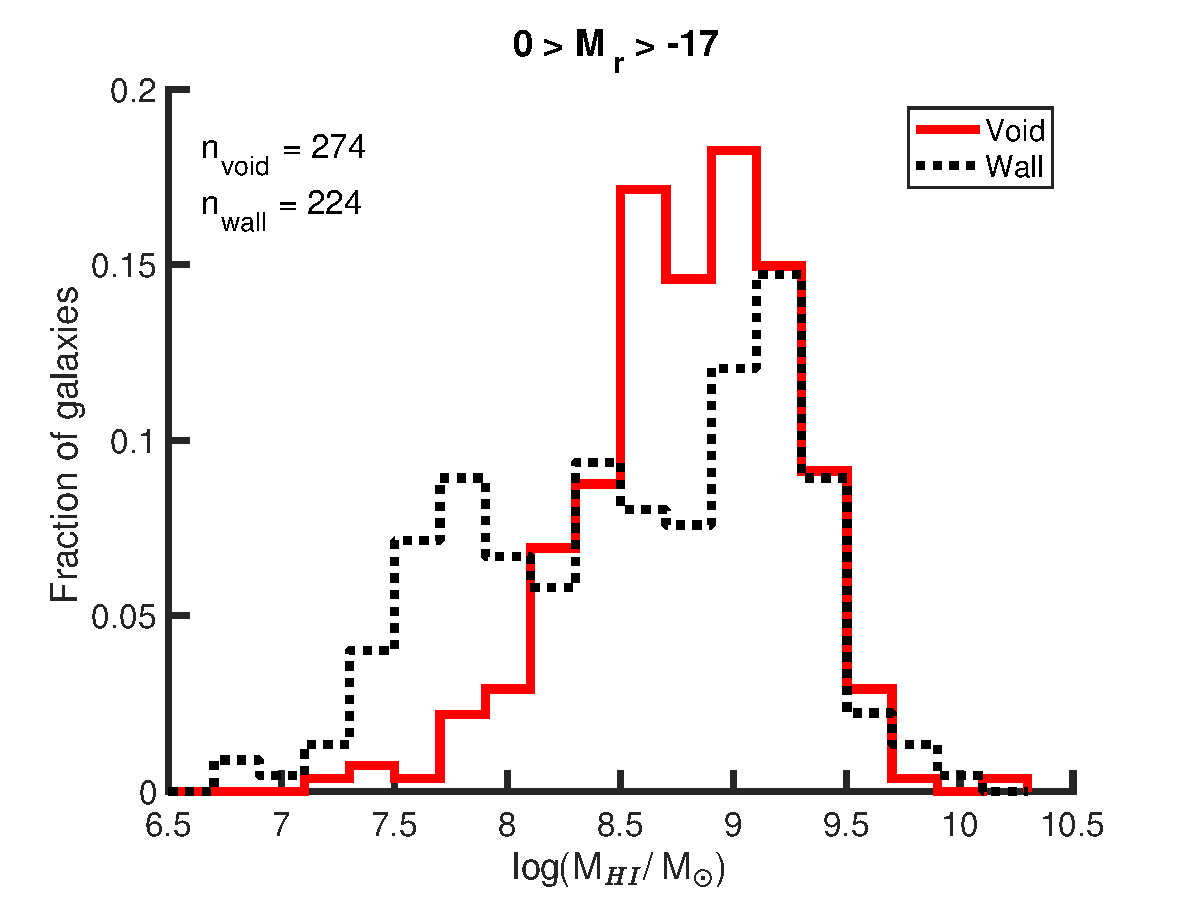
\includegraphics[width=0.49\textwidth]{Images/Paper3/1sig_0-17_I06relations_SF_t3_HI_hist}
    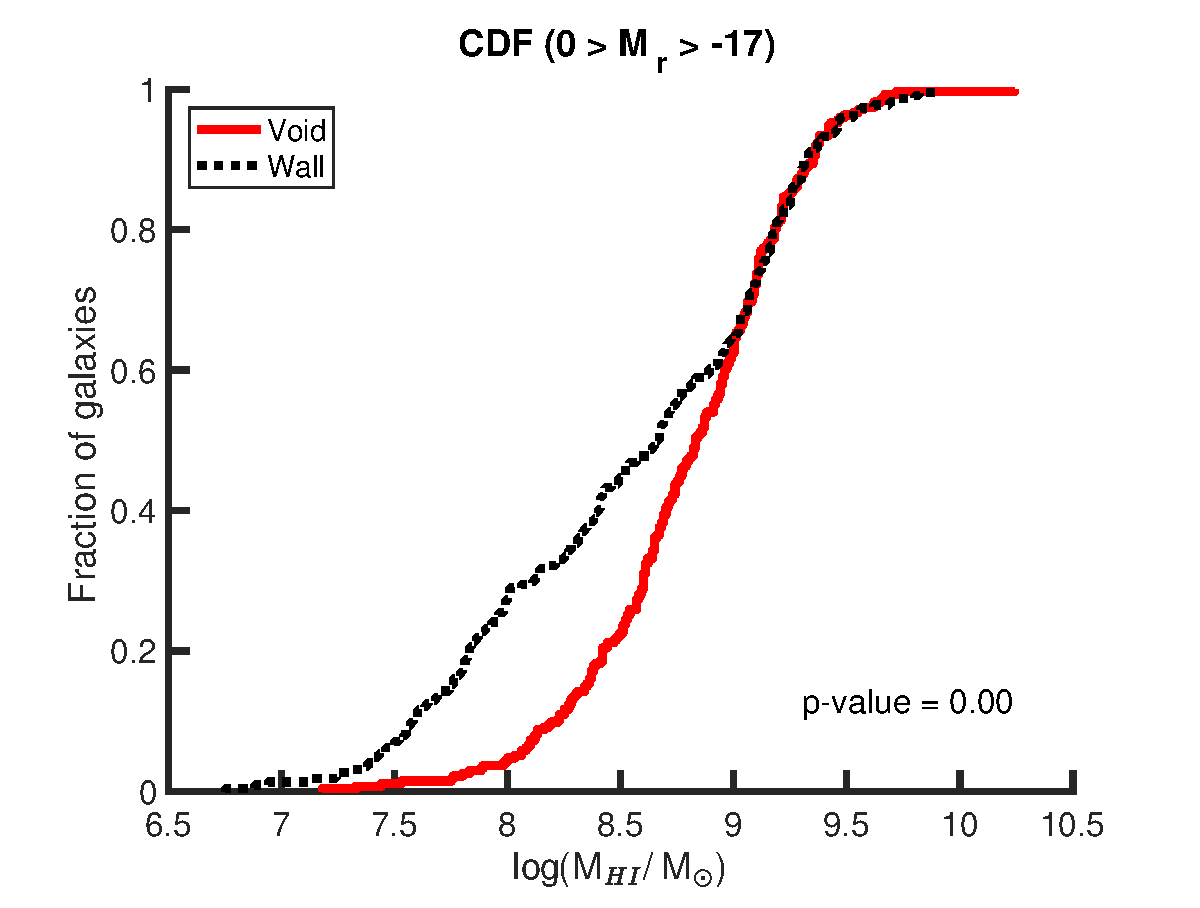
\includegraphics[width=0.49\textwidth]{Images/Paper3/1sig_0-17_I06relations_SF_t3_HI_CDF}
    \caption[\ion{H}{1} mass distribution]{The distribution of \ion{H}{1} mass 
    in the sample of dwarf galaxies, separated by their large-scale environment.  
    There is an obvious shift towards higher \ion{H}{1} masses in the void dwarf 
    galaxies.}
    \label{fig:HI_hist}
\end{figure*}

In addition to looking at the stellar mass, we also investigate the relationship 
between the amount of neutral hydrogen and the gas-phase chemical abundances in 
our sample of star-forming dwarf galaxies.  As shown in \cite{Moorman14}, void 
galaxies typically have lower \ion{H}{1} masses than galaxies in more dense 
regions, consistent with the overall shift of the luminosity or stellar mass 
function to lower luminosity or mass in voids.  In the fixed range of luminosity 
of our dwarf galaxy sample, as Fig. \ref{fig:HI_hist} shows, our sample of void 
dwarf galaxies have higher \ion{H}{1} masses than the dwarf galaxies in denser 
regions.  The gas in the void environment is cooler than that found in denser 
regions (due to less events like shock heating, etc.), which permits void 
galaxies to have higher \ion{H}{1} masses for a given stellar mass.  Therefore, 
because we are fixing the stellar mass in our sample of galaxies (by only 
studying dwarf galaxies), we should find that the void dwarf galaxies have 
higher \ion{H}{1} masses than for those dwarf galaxies in denser environments.

\begin{figure*}
    \centering
    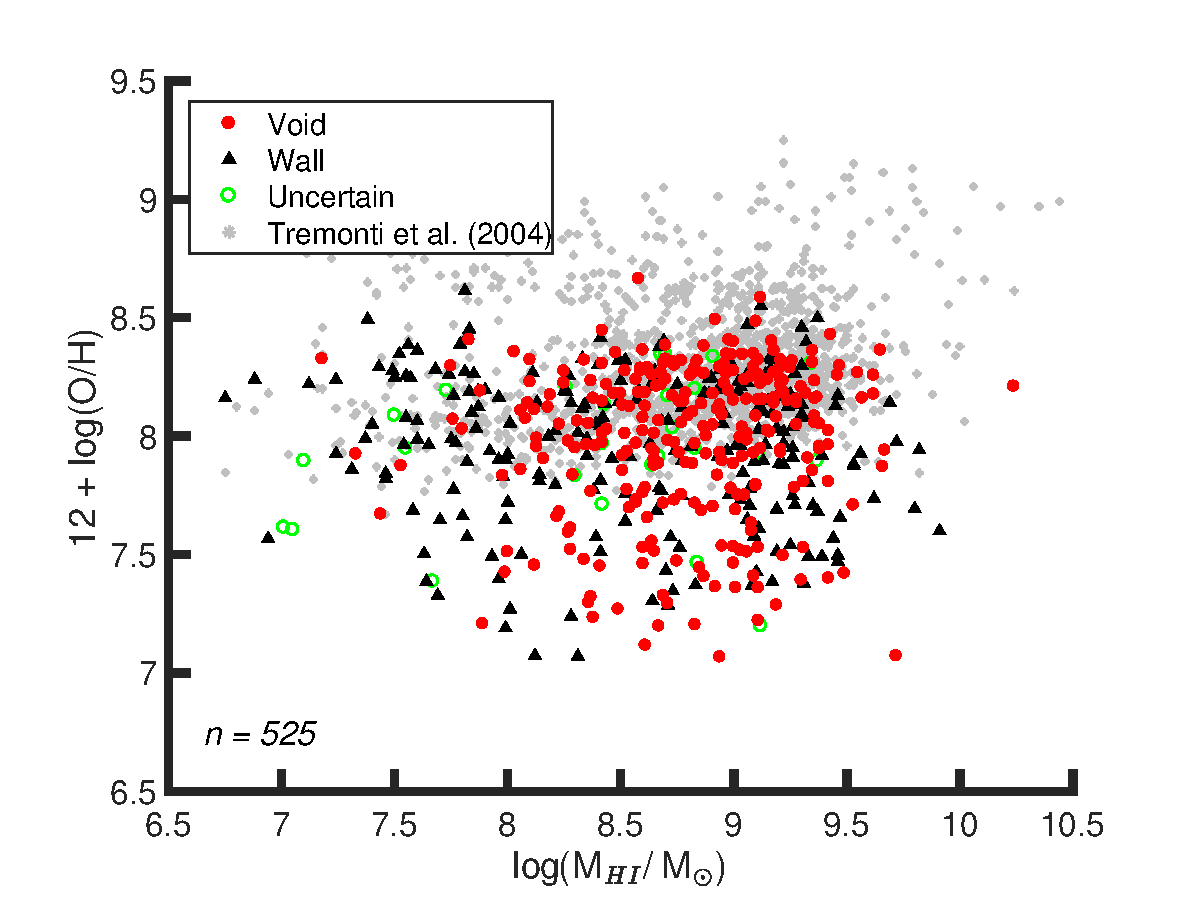
\includegraphics[width=0.49\textwidth]{Images/Paper3/HI_OH_1sig_I06relations_dwarf+T04_SF_t3_dust}
    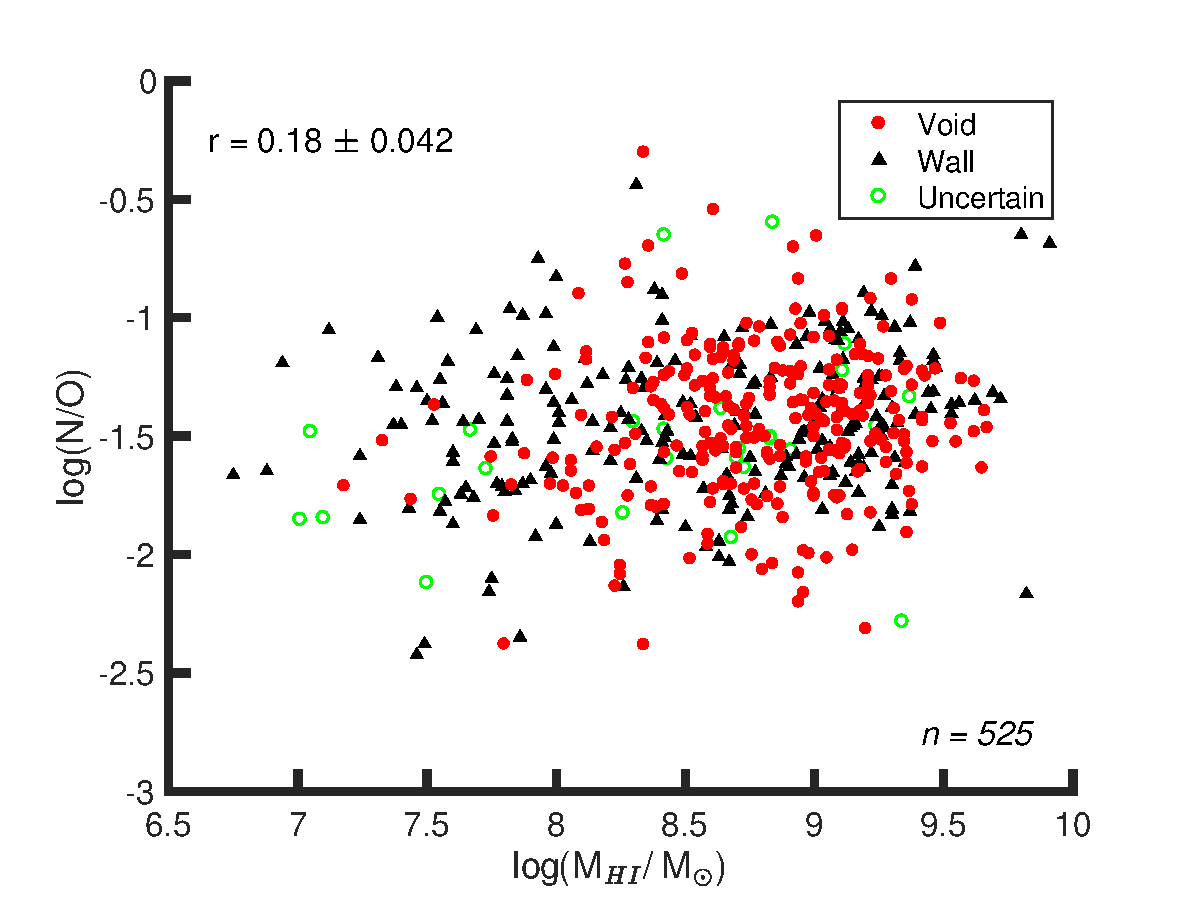
\includegraphics[width=0.49\textwidth]{Images/Paper3/HI_NO_1sig_I06relations_dwarf_SF_t3_dust}
    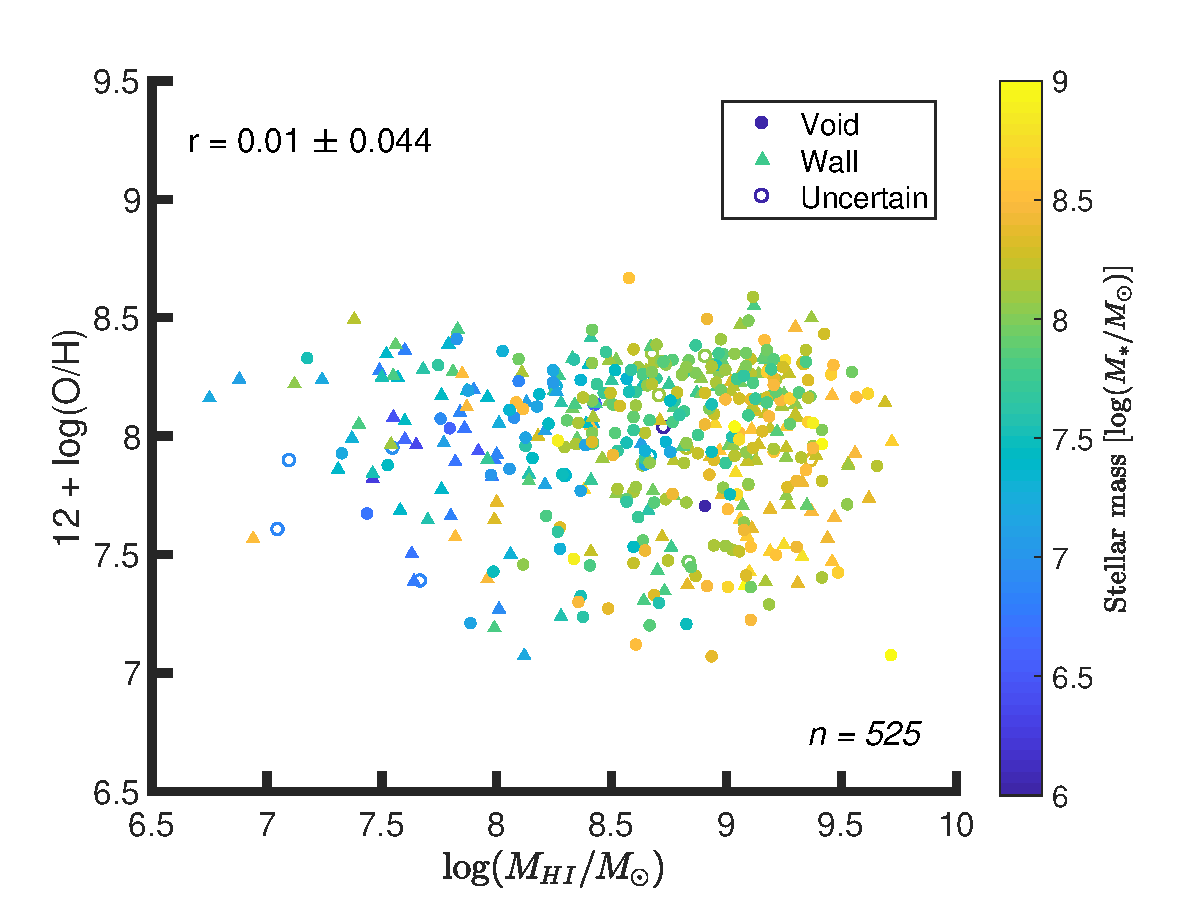
\includegraphics[width=0.49\textwidth]{Images/Paper3/HI_OH_M_1sig_I06relations_dwarf_SF_t3_dust}
    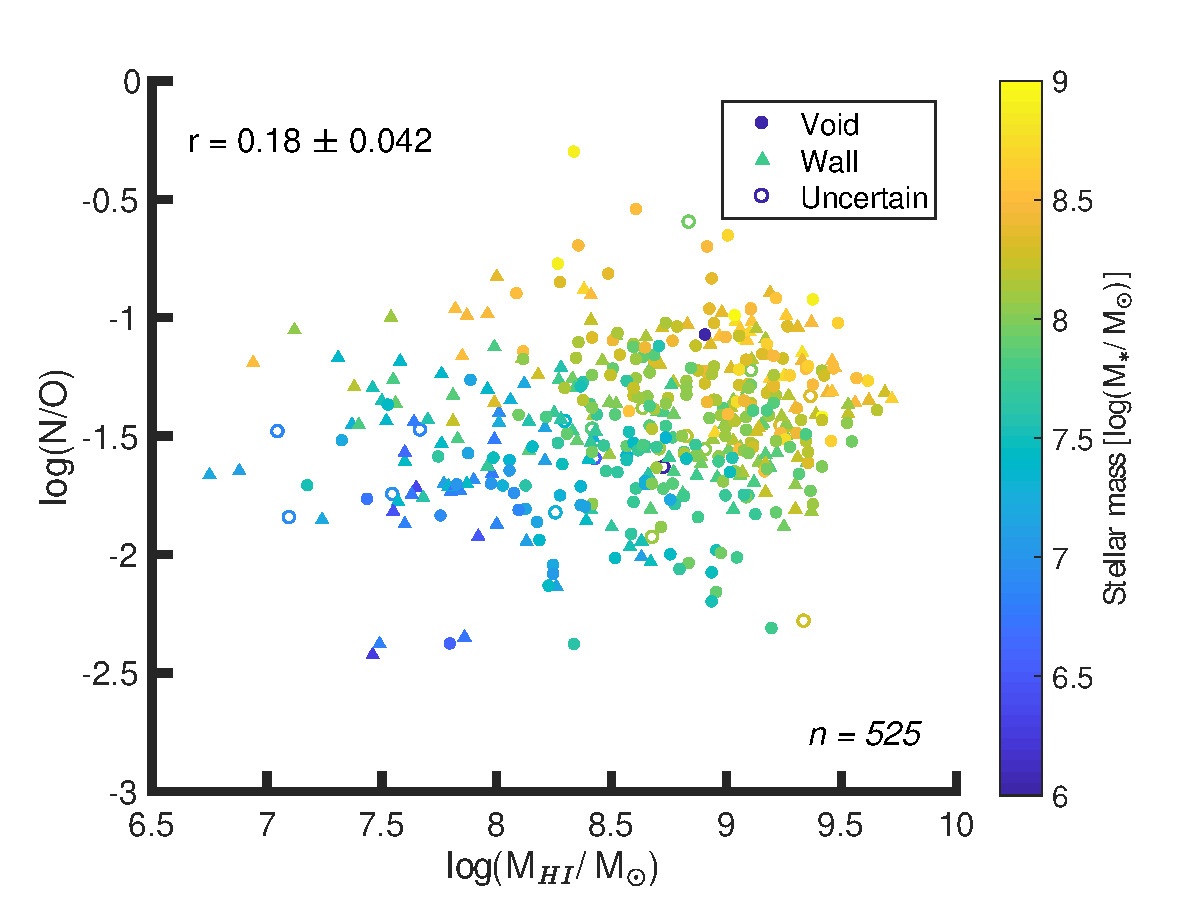
\includegraphics[width=0.49\textwidth]{Images/Paper3/HI_NO_M_1sig_I06relations_dwarf_SF_t3_dust}
    \caption[\ion{H}{1} mass versus O/H and N/O]{\ion{H}{1} mass versus 
    metallicity (left) and N/O ratio (right) for star-forming dwarf galaxies.  
    The color scheme of the top row emphasizes the large-scale environment of 
    the star-forming dwarf galaxies, while the bottom row investigates the 
    relationship between stellar mass, \ion{H}{1} mass, and chemical abundance.  
    Error bars have been omitted for clarity.  To place our oxygen abundance 
    results in context, we show (gray stars) the dwarf galaxies in SDSS DR7 with 
    metallicity estimates from \cite{Tremonti04}.  From these plots, there is no 
    significant influence from the large-scale environment on the relationship 
    between the \ion{H}{1} mass and gas-phase chemical abundances of 
    star-forming dwarf galaxies.}
    \label{fig:HI}
\end{figure*}

The \ion{H}{1} mass-metallicity and \ion{H}{1} mass-N/O relations can be seen in 
Fig. \ref{fig:HI}, extending the results of \cite{Bothwell13} down to 
$\log(M_*/M_\odot) \approx 6$.  Unlike the correlation between the stellar mass 
and the chemical abundances, there is very little correlation between the 
abundances and the \ion{H}{1} mass.  There is no significant relationship 
between the \ion{H}{1} mass and the metallicity of a galaxy --- a linear fit to 
the data in the left panel of Fig. \ref{fig:HI} reveals a slope of only 
$0.05\pm 0.085$ for the void population and $-0.04\pm 0.060$ for the wall 
population.  This is not surprising, as our sample of star-forming dwarf 
galaxies probes the low metallicity range of the MZ relation where there is no 
strong relationship between the metallicity and stellar mass.  There is a very 
small, but statistically significant, relationship between the \ion{H}{1} mass 
and the N/O ratio for the dwarf galaxies: a linear fit to the data in the right 
panel of Fig. \ref{fig:HI} reveals a slope of $0.11\pm 0.083$ for the void dwarf 
galaxies and $0.09\pm 0.060$ for the wall dwarf galaxies.

Due to the time delay in the production of nitrogen relative to oxygen, we 
expect the N/O ratio to decrease with increasing \ion{H}{1} mass, since more 
evolved galaxies have higher N/O ratios and will have used up most of their 
neutral hydrogen.  \cite{Bothwell13} demonstrates the existence of this 
relationship at a fixed stellar mass.  The first row of Fig. \ref{fig:HI} shows 
little, if any, relationship between the \ion{H}{1} mass and the chemical 
abundances.  However, the bottom row of Fig. \ref{fig:HI} shows that there is an 
inverse relationship between the chemical abundance and the \ion{H}{1} mass for 
fixed stellar mass (indicated by the colors of the points).


%-------------------------------------------------------------------------------
\subsection{Color-abundance relations}

\begin{figure*}
    \centering
    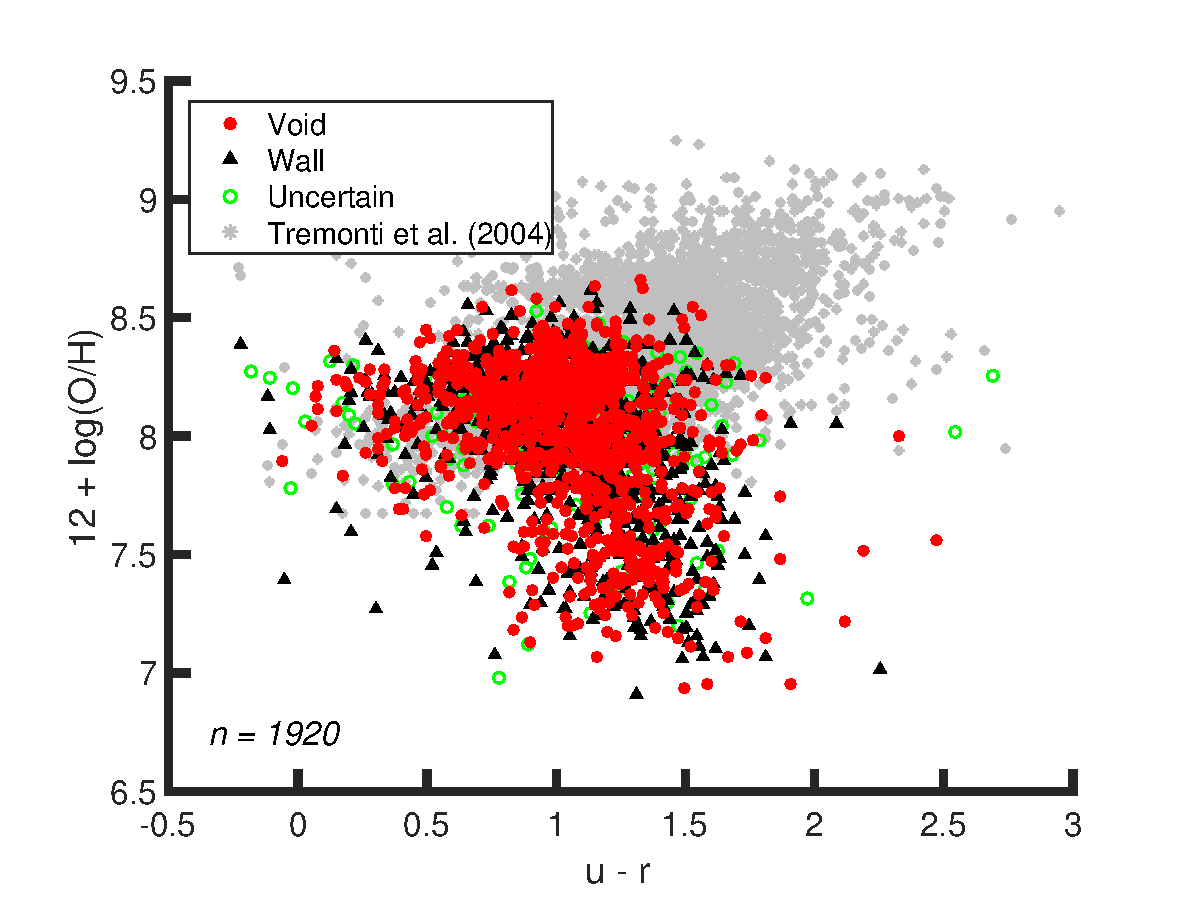
\includegraphics[width=0.49\textwidth]{Images/Paper3/ur_OH_1sig_I06relations_dwarf+T04_SF_t3_dust}
    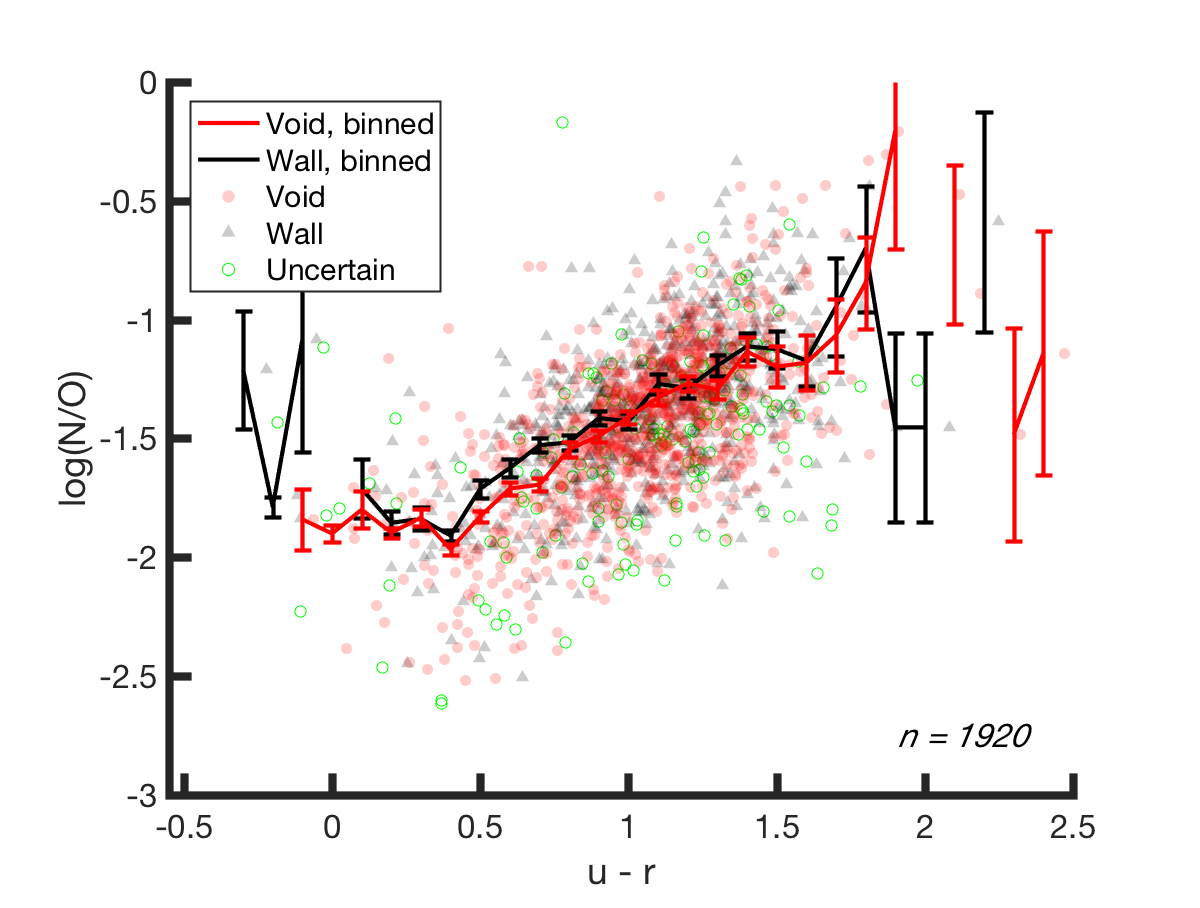
\includegraphics[width=0.49\textwidth]{Images/Paper3/ur_NO_1sig_I06relations_dwarf_SF_t3_dust_scatterURbin}
    \caption[$u-r$ versus O/H and N/O for star-forming dwarf galaxies]{Color 
    ($u-r$) versus the gas-phase oxygen abundance (left) and the N/O ratio 
    (right) for star-forming dwarf galaxies.  Error bars on individual points 
    have been omitted for clarity.  For reference, the dwarf galaxies in SDSS 
    DR7 that have estimated metallicities from \cite{Tremonti04} are shown in 
    the left panel in gray.  To discern any environmental trends in the results, 
    we have binned the galaxies by their color (in bins of width 0.1) on the 
    right.  The large-scale environment does not influence the relationship 
    between the color and chemical abundances of dwarf galaxies.}
    \label{fig:ur_P3}
\end{figure*}

The gas-phase chemical abundance is expected to have a positive correlation with 
a galaxy's color.  Older galaxies have had more time to convert their gas into 
heavier elements through star formation, increasing their metallicities.  The 
color-metallicity and color-N/O relations for our sample of star-forming dwarf 
galaxies can be seen in Figures \ref{fig:ur_P3} and \ref{fig:gr}.  As we see, 
bluer galaxies have lower O/H and N/O ratios when we look at both the $u-r$ and 
$g-r$ colors.  While there is a subset of dwarf galaxies with extremely low 
metallicities that do not follow this trend (seen in the left-hand panels of 
Figures \ref{fig:ur_P3} and \ref{fig:gr}), this population follows the color-N/O 
trend seen on the right in each of these figures.  While these galaxies have 
unusually low oxygen abundances, they have normal N/O ratios.

\begin{figure*}
    \centering
    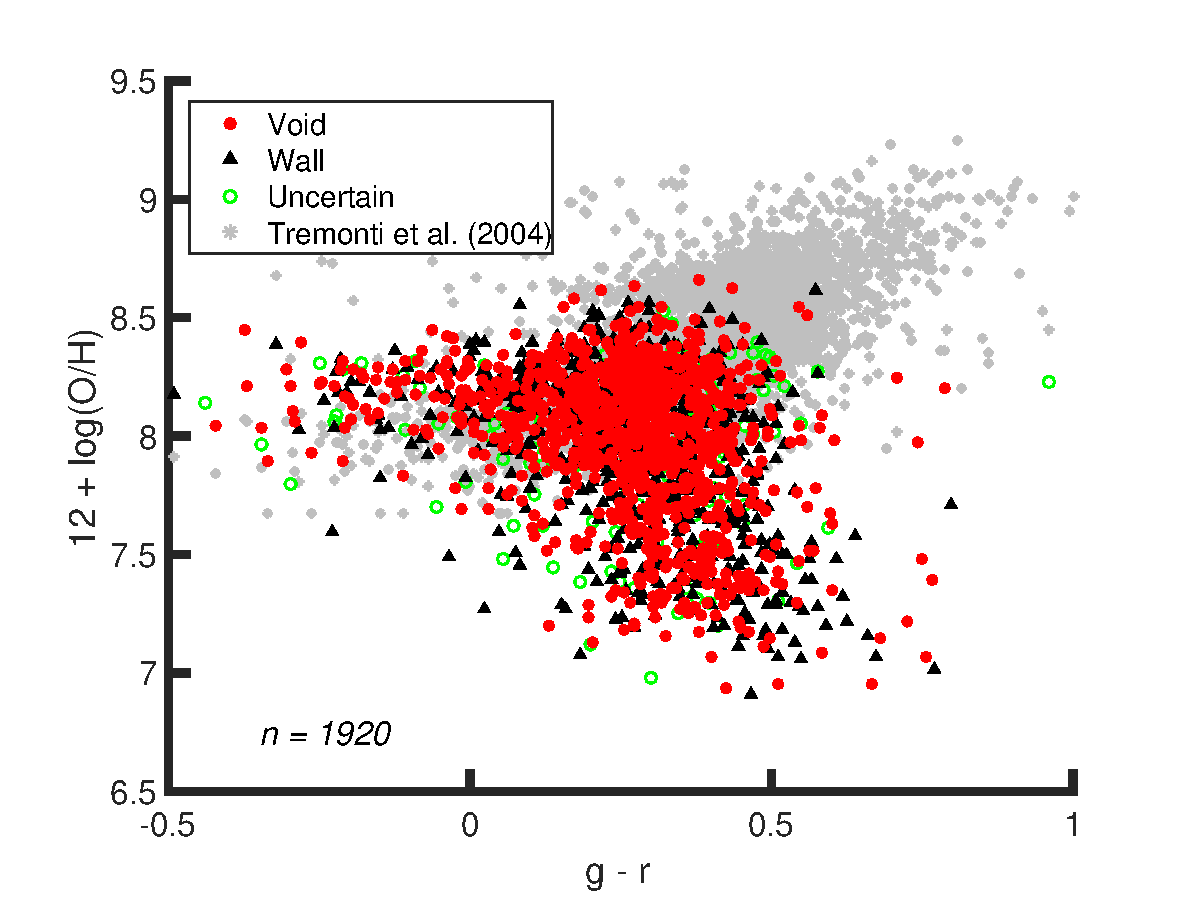
\includegraphics[width=0.49\textwidth]{Images/Paper3/gr_OH_1sig_I06relations_dwarf+T04_SF_t3_dust}
    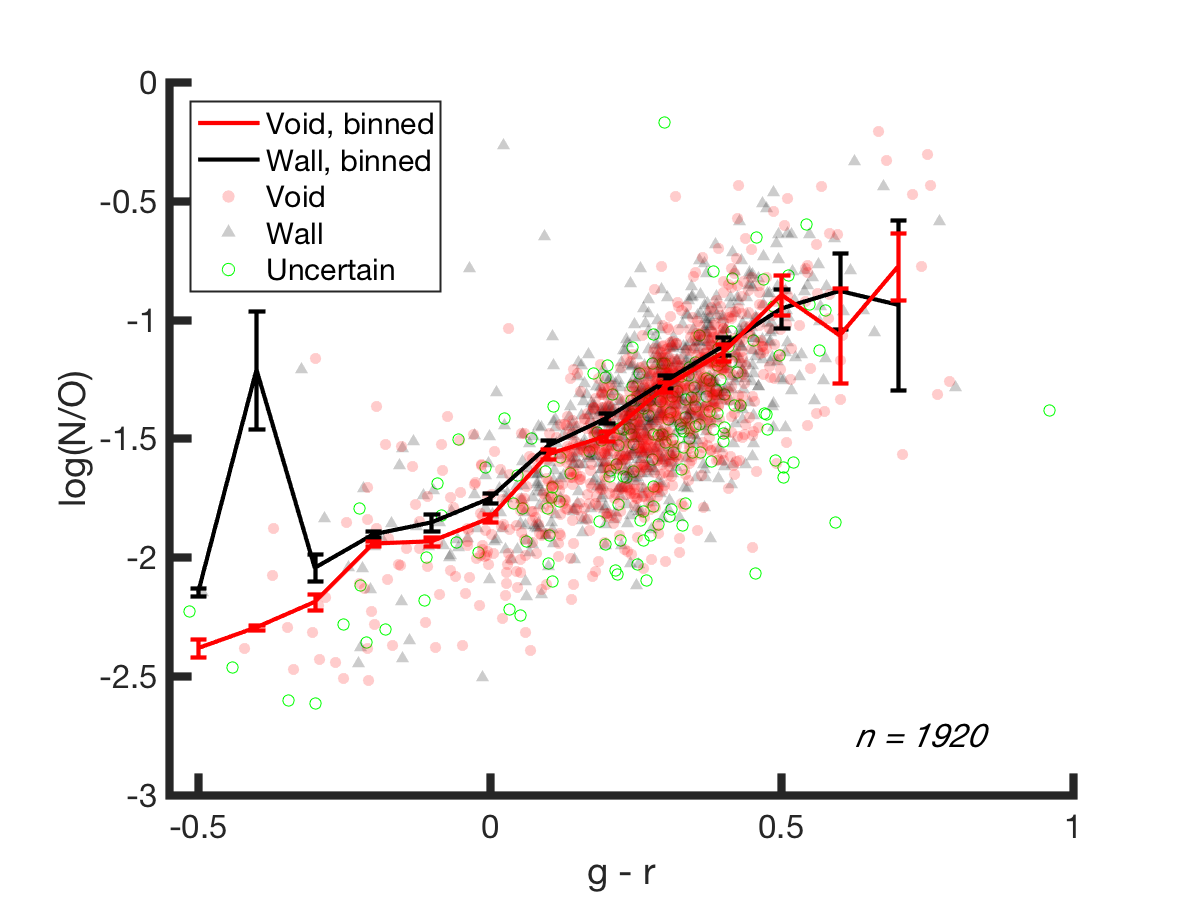
\includegraphics[width=0.49\textwidth]{Images/Paper3/gr_NO_1sig_I06relations_dwarf_SF_t3_dust_scatterGRbin}
    \caption[$g-r$ versus O/H and N/O for star-forming dwarf galaxies]{Color 
    ($g-r$) versus the gas-phase oxygen abundance (left) and the N/O ratio 
    (right) for star-forming dwarf galaxies.  Error bars on individual points 
    have been omitted for clarity.  For reference, the galaxies in SDSS DR7 that 
    have estimated metallicities from \cite{Tremonti04} are shown in the left 
    panel in gray.  To discern any environmental trends in the results, we have 
    binned the galaxies by their color (in bins of width 0.1) on the right.  The 
    large-scale environment does not influence the relationship between the 
    color and chemical abundances of dwarf galaxies.}
    \label{fig:gr}
\end{figure*}

The presence of a relationship between the N/O ratio and the color of a galaxy 
can indicate a time delay between the release of nitrogen and oxygen 
\citep{vanZee06a,Berg12}.  If higher-mass stars are the main source of oxygen, 
then the oxygen will be released on a shorter time scale than nitrogen for a 
given star formation episode (since higher-mass stars turn off the main sequence 
earlier than the intermediate-mass stars that synthesize nitrogen).  Therefore, 
the amount of nitrogen relative to oxygen should increase as the hotter, more 
massive stars burn out and the galaxy becomes redder.  This trend can be seen in 
the star-forming dwarf galaxies on the right of Figures \ref{fig:ur_P3} and 
\ref{fig:gr}, matching the trends seen in \cite{Douglass17b,vanZee06a,Berg12}.

There does not appear to be any influence from the large-scale environment on 
the relationship between the color and chemical abundances for star-forming 
dwarf galaxies.  There is no obvious difference between the void and wall dwarf 
galaxies in the left-hand panels of Figures \ref{fig:ur_P3} and \ref{fig:gr}, 
when we concentrate on the oxygen abundance as a function of color.  To help 
discern any influence from the environment on the N/O ratio as a function of 
color, we bin the star-forming dwarf galaxies by their color in bins of width 
0.1 --- these results are overlaid on the left-hand plots of Figures 
\ref{fig:ur_P3} and \ref{fig:gr}.  The shift toward higher N/O ratios seen in 
the wall bins in both figures is the same shift identified in the histograms in 
Fig. \ref{fig:NOratio_P3}.  Any variation in the color-abundance relationship 
between the void and wall populations except a vertical shift would be evidence 
of the large-scale environment influencing the relationship.  There is a modest 
difference in the slope of these bins in N/O, where the colors of star-forming 
void dwarf galaxies are more strongly correlated with their N/O ratios than 
star-forming wall dwarf galaxies.  The Pearson correlation coefficient between 
$u-r$ and $\log (\text{N}/\text{O})$ for the star-forming void dwarf galaxies is 
$0.63\pm 0.019$ and $0.52\pm 0.027$ for the star-forming wall dwarf galaxies.  
The correlation coefficients between $g-r$ and $\log (\text{N}/\text{O})$ for 
the void dwarf galaxies is $0.74\pm 0.014$ and $0.67\pm 0.020$ for the wall 
dwarf galaxies.  
% What does it mean, for void galaxies to more correlated in their color v. N/O?


%-------------------------------------------------------------------------------
\subsection{(s)SFR-abundance relations}

\begin{figure*}
    \centering
    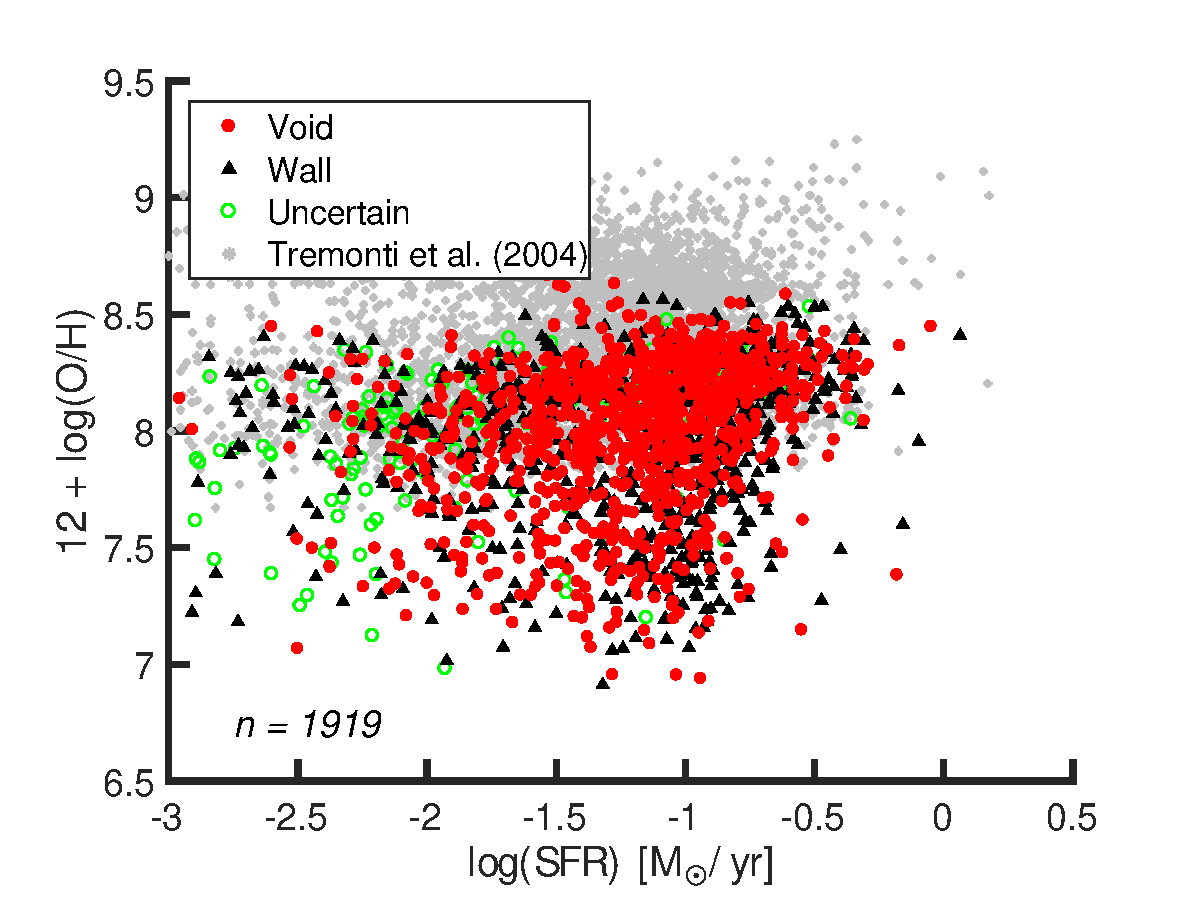
\includegraphics[width=0.49\textwidth]{Images/Paper3/SFR_OH_1sig_I06relations_dwarf+T04_SF_t3_dust}
    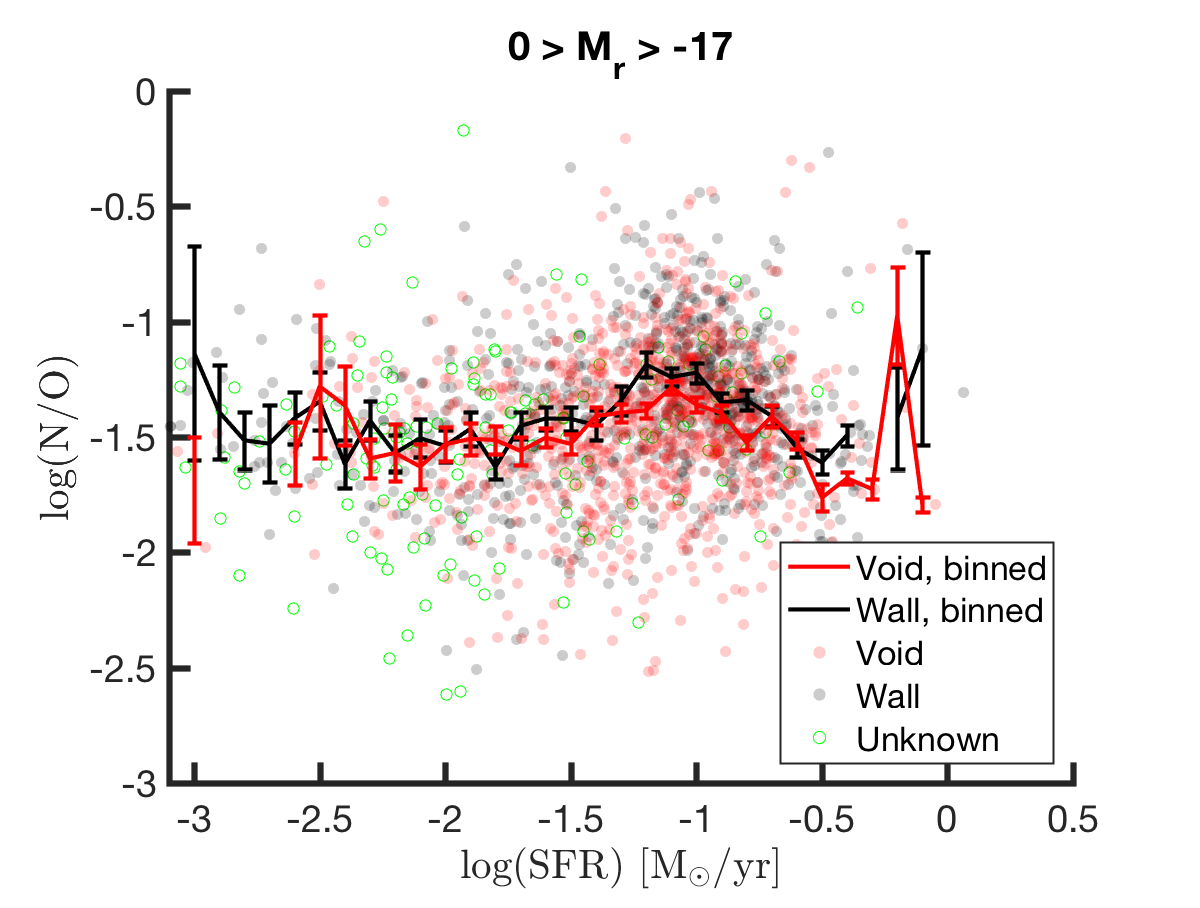
\includegraphics[width=0.49\textwidth]{Images/Paper3/SFR_NO_1sig_I06relations_dwarf_SF_t3_dust_scatterSFRbin}
    \caption[SFR versus O/H and N/O for star-forming dwarf galaxies]{SFR versus 
    metallicity (left) and the N/O ratio (right) for star-forming dwarf 
    galaxies.  Error bars for individual galaxies have been omitted for clarity.  
    To place our oxygen abundance results in context, we show (gray stars) the 
    dwarf galaxies in SDSS DR7 with metallicity estimates from 
    \cite{Tremonti04}.  To discern any environmental effects on the relation 
    between SFR and the N/O ratio, we bin the dwarf galaxies by SFR (in bins of 
    width 0.1).  From these plots, the large-scale environment has no 
    discernible influence on the relationship between the SFR and gas-phase 
    chemical abundances of star-forming dwarf galaxies.}
    \label{fig:SFR}
\end{figure*}

\begin{figure*}
    \centering
    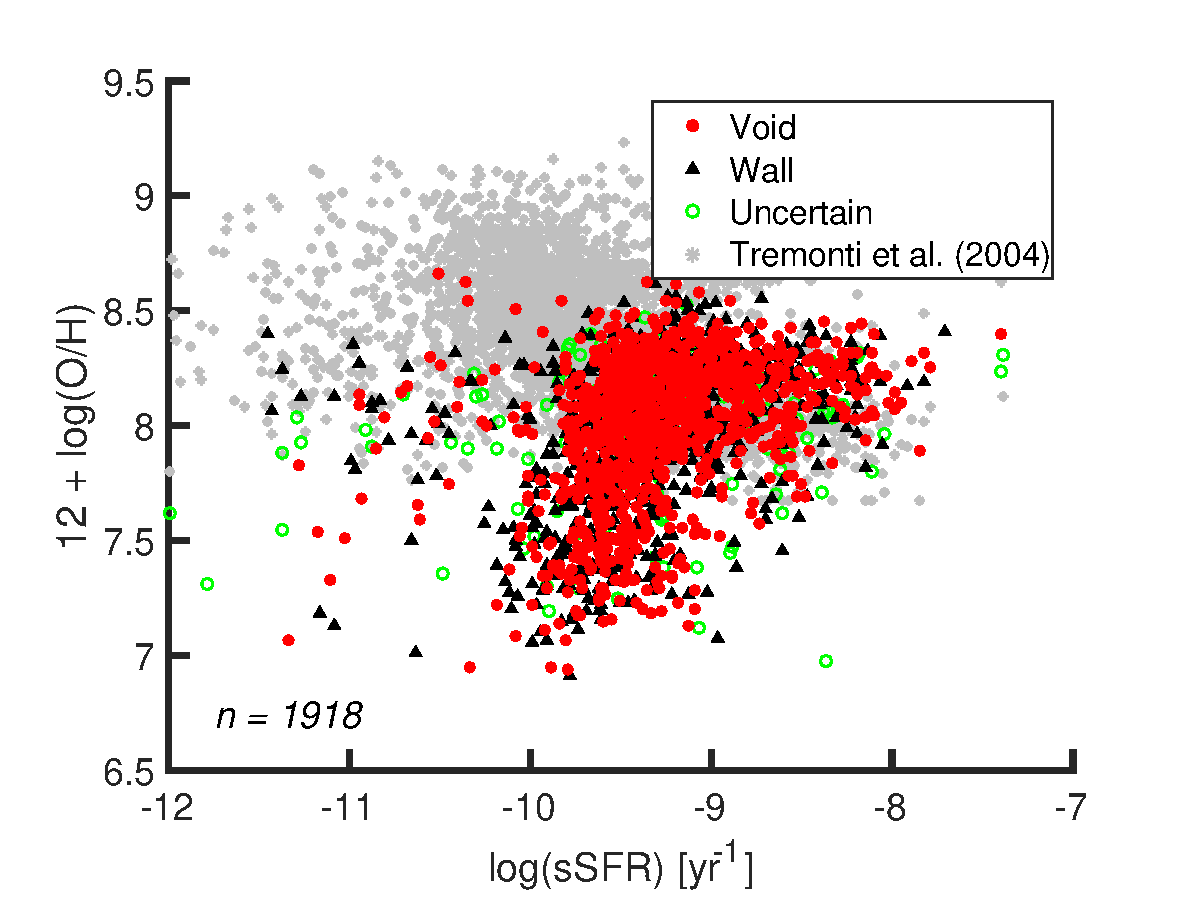
\includegraphics[width=0.49\textwidth]{Images/Paper3/sSFR_OH_1sig_I06relations_dwarf+T04_SF_t3_dust}
    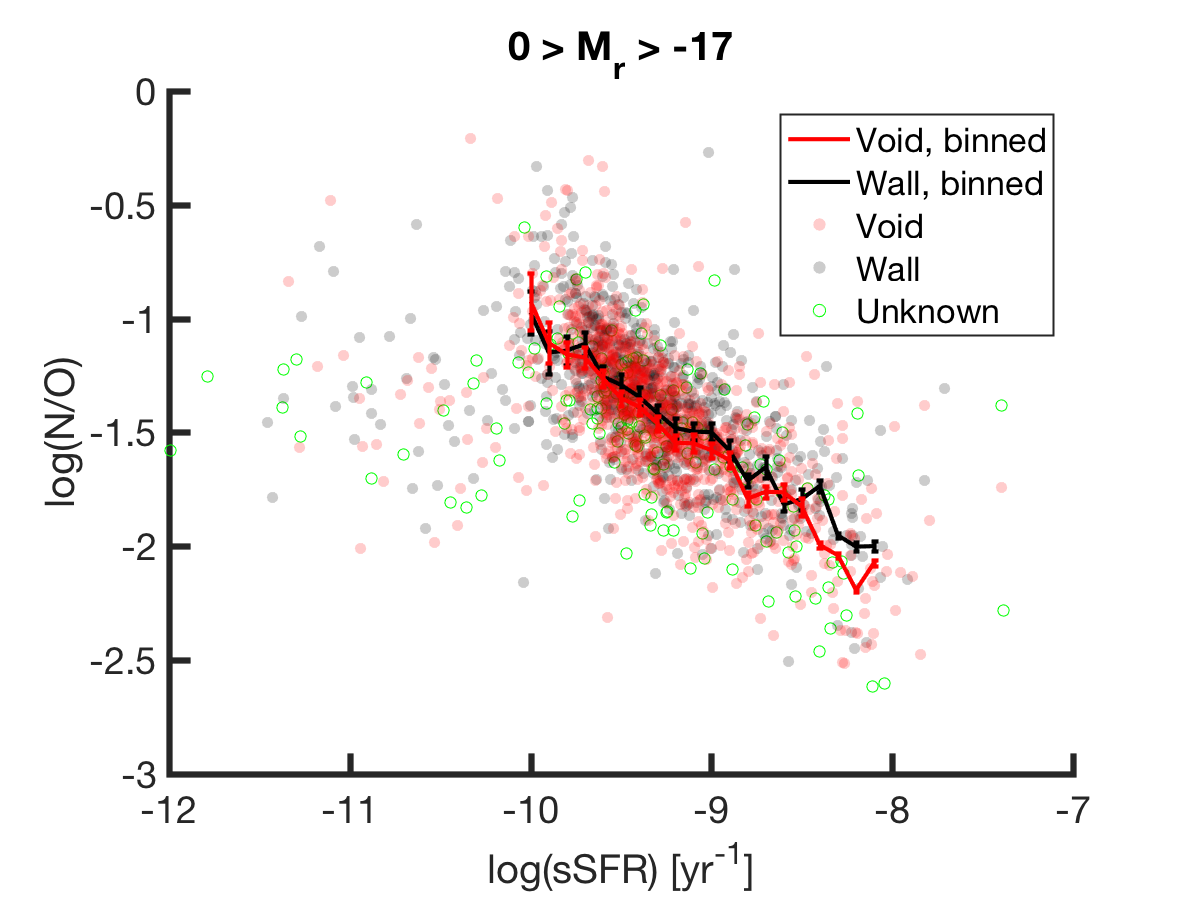
\includegraphics[width=0.49\textwidth]{Images/Paper3/sSFR_NO_1sig_I06relations_dwarf_SF_t3_dust_scattersSFRbin}
    \caption[sSFR versus O/H and N/O for star-forming dwarf galaxies]{Specific 
    star formation rate (sSFR) versus metallicity (left) and the N/O ratio 
    (right) for star-forming dwarf galaxies.  Error bars on individual galaxies 
    have been omitted for clarity.  To place our oxygen abundance results in 
    context, we show (gray stars) the dwarf galaxies in SDSS DR7 with 
    metallicity estimates from \cite{Tremonti04}.  To discern any environmental 
    effects on the relation between sSFR and the N/O ratio, we bin the dwarf 
    galaxies by sSFR (in bins of width 0.1).  From these figures, there is no 
    significant influence on the relationship between the sSFR and gas-phase 
    chemical abundances of star-forming dwarf galaxies.}
    \label{fig:sSFR_P3}
\end{figure*}

There is thought to be a fundamental relationship between the stellar mass, star 
formation rate (SFR), and metallicity of a galaxy \citep{Mannucci10,LaraLopez10,
Andrews13}; the metallicity of a galaxy should increase with stellar mass and 
decrease as a function of the SFR.  \cite{Henry13} observe an inverse 
relationship between the metallicity and SFR of low-mass galaxies.  However, as 
was seen in \cite{Douglass17a}, Fig. \ref{fig:SFR} shows very little correlation 
between the SFR and metallicity or N/O ratio of the star-forming dwarf galaxies.  
When we separate the dwarf galaxies by their large-scale environment, we see no 
difference in the correlation coefficients between the two environments; there 
is no discernible influence on the relationship between the SFR and the chemical 
abundances by the large-scale environment.

We also inspect the relationship between the specific star formation rate (sSFR) 
and the gas-phase chemical abundances in star-forming dwarf galaxies.  As shown 
in Fig. \ref{fig:sSFR_P3}, there is a stronger correlation between the sSFR of a 
dwarf galaxy and its metallicity and N/O ratio.  The left-hand panel of Fig. 
\ref{fig:sSFR_P3} shows the relationship between the gas-phase oxygen abundance 
and the sSFR for star-forming dwarf galaxies; to place our results in context, 
we also include (gray stars) those dwarf galaxies in SDSS DR7 for which 
\cite{Tremonti04} was able to estimate metallicities.  In the metallicity regime 
we are able to probe (\OH $\leq 8.5$), the star-forming dwarf galaxies display 
relatively little relationship between their sSFR and metallicity.  The group of 
extremely low metallicity dwarf galaxies (\OH $< 7.6$) in our sample has some of 
the lowest sSFR of our dwarf galaxies.

As we see on the right in Fig. \ref{fig:sSFR_P3}, though, there is a strong 
anti-correlation between the sSFR and N/O ratio for the star-forming dwarf 
galaxies.  Galaxies with higher sSFRs may be producing more massive stars than 
galaxies with lower sSFRs.  If oxygen is produced in more massive stars than 
those which produce nitrogen, then the galaxies with higher sSFRs will produce 
more oxygen earlier than those galaxies with lower sSFRs.  Increasing the 
gas-phase oxygen abundance relative to nitrogen will decrease the N/O ratio in 
these galaxies with higher sSFRs.  Therefore, an anti-correlation between the 
sSFR and N/O ratio is further evidence that oxygen is produced in higher mass 
stars than those which synthesize nitrogen.

There is also very little scatter in the right-hand panel of Fig. 
\ref{fig:sSFR_P3}, indicating a significant relationship between the sSFR and 
N/O ratio for dwarf galaxies.  The Pearson correlation coefficients for our 
sample of star-forming void dwarf galaxies is $-0.62\pm 0.020$; the correlation 
coefficient for the star-forming wall dwarf galaxies is $-0.55\pm 0.025$.  It is 
interesting to note that the void dwarf galaxies exhibit a stronger correlation 
between their sSFR and N/O ratio than the dwarf galaxies in denser environments.  
This can be seen in the binned data points plotted on top of the individual 
dwarf galaxies; we have taken the average of the galaxies binned by their sSFR 
(in bins of width 0.1) to help discern any large-scale environmental influence 
on the relationship between the sSFR and the N/O ratio.
% Again, what is the physical interpretation of the stronger correlation in the void galaxies?



%%%%%%%%%%%%%%%%%%%%%%%%%%%%%%%%%%%%%%%%%%%%%%%%%%%%%%%%%%%%%%%%%%%%%%%%%%%%%%%%
%
%    DISCUSSION
%
%%%%%%%%%%%%%%%%%%%%%%%%%%%%%%%%%%%%%%%%%%%%%%%%%%%%%%%%%%%%%%%%%%%%%%%%%%%%%%%%
\section[Environmental influence]{Large-scale environmental influence}

We see small, statistically significant shifts in each of the three gas-phase 
abundance ratios studied as a function of the large-scale environment, implying 
that the large-scale environment influences the chemical abundances of 
star-forming dwarf galaxies.  Previous work by \cite{Douglass17b} suggests that 
the oxygen abundance (O/H), nitrogen abundance (N/H), and N/O ratio depend on a 
galaxy's environment.  Work by \cite{Shields91} finds no shift in the N/O ratio 
between cluster and field galaxies, though they do find that cluster galaxies 
have higher metallicities than field galaxies.  \cite{Contini02} and 
\cite{Pilyugin02} find a statistically insignificant shift in the N/O ratio 
between cluster and field galaxies, where cluster galaxies have lower N/O ratios 
than field spiral galaxies.  The shifts seen in each of these latter three 
sources are opposite to what we observe in this paper, though these previous 
studies concentrate on the galaxies in the Virgo cluster, which are more massive 
than our dwarf galaxy ($M_r > -17$) sample.  On average, we find that 
star-forming void dwarf galaxies have $\sim$7\% higher oxygen abundances, 
$\sim$10\% lower nitrogen abundances, and $\sim$17\% lower N/O ratios than 
star-forming dwarf galaxies in denser regions.

As outlined in \cite{Douglass17a}, there have been numerous previous studies 
that investigate the influence of the environment on the metallicity of a 
galaxy, resulting in mixed conclusions.  When a difference in the metallicity 
was attributed to the environment \citep[as in][for example]{Pustilnik06,
Pustilnik11b,Pustilnik14,SanchezAlmeida16,Cooper08}, it was found that those 
galaxies with higher metallicities preferentially reside in denser regions.  
This is the opposite of the trend seen in Fig. \ref{fig:met1sig_P3} in the 
star-forming dwarf galaxies, although our results are not a direct comparison 
with their conclusions (do to our requirement of the [\ion{O}{3}] $\lambda$4363 
auroral line, we are not able to probe the high-metallicity regime).  We observe 
an average metallicity that is $\sim$7\% higher in void dwarf galaxies than in 
dwarf galaxies in denser regions.


\subsection{Higher metallicities in void dwarf galaxies}

% The direction of the shift implies more O in voids
%  - How do we get more O in void galaxies?  M_DM/M_* |v > M_DM/M_* |w
We posit that the slightly higher metallicities seen in the star-forming void 
dwarf galaxies in Fig. \ref{fig:met1sig_P3} is due to a large-scale 
environmental effect on the ratio of a galaxy's dark matter halo mass to stellar 
mass ($M_{DM}/M_*$).  \cite{Goldberg04} show that gravitational clustering 
within a void proceeds as if in a very low density universe, where the growth of 
gravitationally bound dark matter halos ends relatively early.  Afterwards, 
there is relatively little interaction between the void galaxies because of the 
lower density and faster local Hubble expansion.  Simulations by \cite{Jung14} 
and \cite{Tonnesen15} show that, for a fixed dark matter halo mass, the stellar 
masses of central galaxies located in voids are smaller than those of central 
galaxies living in denser regions.  The $\Lambda$CDM cosmology predicts that 
galaxies formed in voids will be retarded in their star formation when compared 
to those in denser environments.  Therefore, void dwarf galaxies could have 
higher $M_{DM}/M_*$ ratios than dwarf galaxies in denser regions.

If this is the case, then the potential well and virial radius of the void 
galaxies are large enough to retain more of the heavy elements that are blown 
from the ISM to the CGM of a galaxy (from a supernova, for example).  The 
simulation results of \cite{Tonnesen15} find that, for central galaxies with 
halo masses between $10^{11}$ and $10^{12.9}$, void galaxies have $\sim$10\% 
larger ratios of dark matter halo mass to stellar mass than wall galaxies at 
$z = 0$.  In wall galaxies, more of these heavy elements can escape the dwarf 
galaxy, while in void galaxies they are confined to the CGM and eventually fall 
back onto the galaxy's ISM.  If star-forming void dwarf galaxies are able to 
retain more oxygen relative to their hydrogen abundance, then they will reach 
the critical value of O/H for secondary nitrogen production (via the CNO cycle) 
earlier than the star-forming wall dwarf galaxies, for a given stellar mass.  We 
see this in Fig. \ref{fig:M_NO}, where the N/O plateau for the void dwarf 
galaxies exists for stellar masses $\log(M_*/M_\odot) \lesssim 7.2$.  In 
contrast, the N/O plateau for the wall dwarf galaxies exists for stellar masses 
$\log(M_*/M_\odot) \lesssim 7.6$.

% What other proof do we have that this might be true?
If void dwarf galaxies have higher $M_{DM}/M_*$ ratios than dwarf galaxies in 
denser environments, we would expect to see an environmental influence on other 
characteristics of these galaxies.  First, the ratio of neutral hydrogen mass to 
stellar mass of the dwarf galaxies would be higher in star-forming void galaxies 
than star-forming wall galaxies, under the assumption that neutral hydrogen 
traces dark matter.  We see this effect both in Fig. 9 of \cite{Moorman16} and 
in Fig. \ref{fig:HI_hist} above.  Second, the \ion{H}{1} mass function should 
shift less from wall to void galaxies than the shift seen in the luminosity 
function.  Indeed, \cite{Moorman16} finds a shift of characteristic \ion{H}{1} 
mass by a factor of 1.4 in the \ion{H}{1} mass function, while \cite{Hoyle05} 
measures a shift by a factor of 2.5 in luminosity in the luminosity function 
between these two environments.


\subsection{Lower N/O ratios in void dwarf galaxies}

% Shift in N/O due to environmental influence on cosmic downsizing
As we see in Fig. \ref{fig:NOratio_P3}, star-forming void dwarf galaxies have a 
lower N/O ratio than wall dwarf galaxies.  This strengthens the preliminary 
results found in \cite{Douglass17b} and the simulation results of \cite{Cen11}, 
indicating that void galaxies are retarded in their star formation and that 
cosmic downsizing might depend on the large-scale environment.  As suggested by 
\cite{vanZee06a}, a galaxy with a declining SFR at late times (a wall galaxy) 
will have a higher N/O ratio than a galaxy with a constant SFR (a void galaxy); 
the ongoing star formation in the void galaxies will release more oxygen into 
the ISM, decreasing their N/O ratio relative to the galaxies with declining 
SFRs.  This concept is supported by the color-N/O diagram in Figures 
\ref{fig:ur_P3} and \ref{fig:gr}, where the bluer galaxies have lower N/O 
ratios.  The correlations between color and the N/O ratio found in 
\cite{vanZee06a}, \cite{Berg12}, \cite{Douglass17b}, and this work are a result 
of declining SFRs \citep{vanZee06a}.  The average lower N/O ratios we see in 
star-forming void dwarf galaxies may be observational evidence that cosmic 
downsizing is environmentally dependent.


\subsection{Extremely low metallicity dwarf galaxies}

Previous studies have either hypothesized \citep{Pustilnik06,Pustilnik11b,
Pustilnik13} or concluded \citep{Filho15} that low-metallicity objects 
preferentially reside in low-density environments.  \cite{Douglass17a} find 
that, out of 135 dwarf galaxies studied, there is no difference in the fraction 
of low-metallicity dwarf galaxies that reside in voids and denser regions.  Of 
the 1920 dwarf galaxies we analyze, 287 have extremely low metallicity values 
(\OH $\leq 7.6$).  Of these 287 low-metallicity dwarf galaxies, 144 are found in 
voids (approximately 15\% of the star-forming void dwarf galaxy population 
studied) and 122 are located in denser regions (16\% of the star-forming wall 
dwarf galaxy population studied).  These population fractions do not support the 
existence of a special population of extremely metal-poor dwarf galaxies in 
voids.

We find that these 287 extremely metal-poor galaxies are only slightly lower in 
their nitrogen abundances when compared to the total star-forming dwarf galaxy 
population studied.  The low oxygen abundances causes these dwarf galaxies to 
have higher N/O ratios than the total star-forming dwarf galaxy population 
studied.  From Figures \ref{fig:ur_P3} and \ref{fig:gr}, it is apparent that 
these extremely metal-poor star-forming dwarf galaxies are redder than their 
oxygen abundances would typically indicate, although their colors align with 
their N/O ratios.  Fig. \ref{fig:SFR} also shows that the sSFRs for these 
low-metallicity dwarf galaxies are lower than expected for their oxygen 
abundances, though their sSFRs conform with the observed relationship between 
the N/O ratio and the sSFR.  The 287 extremely metal-poor galaxies are isolated 
from our main sample of star-forming dwarf galaxies only when comparing their 
gas-phase oxygen abundances to other physical characteristics; their N/O ratios 
are not unusual.


%%%%%%%%%%%%%%%%%%%%%%%%%%%%%%%%%%%%%%%%%%%%%%%%%%%%%%%%%%%%%%%%%%%%%%%%%%%%%%%%
%
%    CONCLUSION
%
%%%%%%%%%%%%%%%%%%%%%%%%%%%%%%%%%%%%%%%%%%%%%%%%%%%%%%%%%%%%%%%%%%%%%%%%%%%%%%%%
\section{Conclusions}

% Need a topic sentence that refers back to the introduction
We estimate the gas-phase oxygen and nitrogen abundances and the N/O ratio of 
star-forming dwarf galaxies in SDSS DR7 using the direct $T_e$ method and 
spectroscopic line flux measurements as reprocessed in the MPA-JHU catalog.  We 
expand upon the previous work of \cite{Douglass17a} and \cite{Douglass17b} by 
deriving a relation between the doubly-ionized oxygen and total oxygen abundance 
in star-forming galaxies; removing the dependence on the [\ion{O}{3}] 
$\lambda$3727 doublet, this relation allows us to probe those dwarf galaxies at 
$z < 0.02$ in SDSS DR7.  The 1920 dwarf galaxies analyzed indicate that the 
large-scale environment influences their chemical evolution: star-forming void 
dwarf galaxies have higher oxygen abundances by an average of 7\%, lower 
nitrogen abundances by an average of 10\%, and 17\% lower N/O ratios than 
star-forming dwarf galaxies in denser regions.  The large-scale ($\sim$10 \hMpc) 
environment influences the chemical evolution of star-forming dwarf galaxies.

% Summary of comparison with physical characteristics
In addition, we also look at the relationship between the metallicity and the 
N/O ratio and other physical characteristics of our star-forming dwarf galaxy 
sample.  In the relationship between N/O and O/H, all our dwarf galaxies reside 
on the so-called ``nitrogen plateau,'' where the N/O ratio is predicted to be 
independent of the gas-phase oxygen abundance for metallicities \OH $< 8.5$.  
Instead of a constant value for the N/O ratio, we instead find that the N/O 
ratio decreases with increasing metallicity.  However, we do find a plateau in 
our relationship between the stellar mass and N/O ratio.  Most of our 
star-forming dwarf galaxies follow the typical mass-metallicity relation 
\citep{Tremonti04}.  There is no relationship between the metallicity and 
\ion{H}{1} mass of the galaxies, but the N/O ratio decreases with increasing 
\ion{H}{1} mass for fixed stellar mass.  The star-forming dwarf galaxies exhibit 
an increase in the metallicity (O/H) and N/O ratio with increasing color (both 
$u-r$ and $g-r$).  We see very little correlation with SFR for either 
metallicity (O/H) or N/O ratio of dwarf galaxies, but the metallicity and N/O 
ratio decrease with increasing sSFR.  Beyond the large-scale environmental 
influence on the chemical abundance distributions in the sample of star-forming 
dwarf galaxies, we do not observe any significant differences between the 
star-forming void and wall dwarf galaxies in any of these relationships.

% Physical interpretation for the shift in O/H, N/O
We surmise that the differences in the distributions of metallicity and the N/O 
ratio seen in the sample of star-forming dwarf galaxies are due to a large-scale 
environmental influence on their formation history and evolution.  The shift in 
the gas-phase oxygen abundance distribution could be observational evidence for 
delayed star formation in void galaxies when compared to those in denser 
regions.  This would result in a smaller ratio of stellar mass to dark matter 
halo mass in void galaxies than in wall dwarf galaxies, as predicted in 
simulations by \cite{Jung14} and \cite{Tonnesen15}.  Simulations looking at how 
the retention fraction of supernovae ejecta depends on the halo mass or dark 
matter potential would be useful in understanding if a $\sim$10\% increase in 
the dark matter halo mass for void dwarf galaxies is enough to result in a 
$\sim$7\% increase in the metallicity.  If the void galaxies are retaining more 
oxygen as a result of their deeper potential wells, then they will be able to 
commence the synthesis of secondary nitrogen earlier, as is seen in the mass-N/O 
relation in Fig. \ref{fig:M_NO}.  In addition, the shift towards lower N/O 
ratios in the star-forming void dwarf galaxies may be evidence that cosmological 
downsizing is environmentally dependent.  Our results provide evidence for 
delayed, ongoing star formation in void dwarf galaxies whose dark matter halos 
ceased coalescing earlier than for dwarf galaxies in denser regions.

% XMP dwarf galaxies
No special population of extremely metal-poor star-forming dwarf galaxies is 
found in the voids, as we note an equal fraction of low metallicity dwarf 
galaxies in both the voids and denser regions.  Due to their low gas-phase 
oxygen abundances, the 287 dwarf galaxies have some of the larger N/O ratios of 
the star-forming dwarf galaxy sample studied.  While the metallicities of these 
galaxies cause them to stand out when looking at the relationship between the 
metallicity and other physical characteristics of the galaxies (stellar mass, 
color, (s)SFR), they are not unusual when studying the relationship between the 
N/O ratio and the other galaxy properties.